\documentclass{article}

\usepackage{hyperref}
\usepackage{tocloft}
\usepackage[left=2.5cm,right=2.5cm,top=2.5cm,bottom=2.5cm]{geometry}
\usepackage{fancyhdr}
\usepackage{listings}
\usepackage{xcolor}
\usepackage{amsmath}
\usepackage{graphicx}
\usepackage{listings} % Paket für Quellcode-Listings



\pagestyle{fancy}
\fancyhf{}
\fancyhead[L]{Aufgabe 3}
\fancyhead[R]{Teilnehmer-ID:}
\fancyfoot[C]{\thepage}

\renewcommand{\cftsecleader}{\cftdotfill{\cftdotsep}}
\renewcommand*\contentsname{Inhaltsverzeichnis}

\title{\Huge{\textbf{Aufgabe 3 Siedler}} \\ \centering{\LARGE{Teilnahme-ID: ?????}}}
\author{Bearbeiter dieser Aufgabe: \\ Daniel Hohmann}
\date{\today}

\begin{document}
% Konfiguration für C++-Code
\lstset{
    language=C++, % Sprache des Codes
    basicstyle=\small\ttfamily, % Grundschriftart und -größe
    keywordstyle=\color{blue}\bfseries, % Stil für Schlüsselwörter
    commentstyle=\color{green!60!black}, % Stil für Kommentare
    stringstyle=\color{red}, % Stil für Zeichenketten
    breaklines=true, % Automatischer Zeilenumbruch
    showstringspaces=false, % Keine Leerzeichen in Zeichenketten anzeigen
    tabsize=2, % Tabulatorgröße
    numbers=left, % Zeilennummern links anzeigen
    numberstyle=\tiny\color{gray}, % Stil für Zeilennummern
    captionpos=b % Position der Beschriftung (unten)
}

\thispagestyle{empty}
\begin{center}
\Huge{\textbf{Aufgabe 1 Siedler}}
\\
\LARGE{Teilnehmer-ID: ???}
\\
\LARGE{Bearbeiter dieser Aufgabe: \\ Daniel Hohmann}
\\
\LARGE{\today}
\end{center}
\newpage
\setcounter{page}{1}
\tableofcontents
\newpage
\section{\textcolor{blue}{Loesungsidee}}
\begin{center}
Ich habe mir die Aufgabe durchgelesen, und dabei gemerkt, dass die Hauptaufgabe im Endefekt nichts anderes ist, wie die den Punkt im polygon zu finden, der wen ich mein radius von 85km platziere, die meisten Doerfer im abstand von 10km halten kann. Danach muss ich im endefekt nur noch die restlichen Doerfer im abstand von 20km platzieren.
\end{center}
\section{\textcolor{blue}{Umsetzung}}
\subsection{\textcolor{blue}{Erste schritte und fehler}}
\subsubsection{\textcolor{blue}{raster algorithmus}}
\begin{center}
ich habe viele probleme mit der umsetzung. Das groeste problem ist es, den optimalsten punkt innerhalb des polygons zu finden. So das ich moeglichst viele doerfer im abstand von 10km platzieren kann.
\par\medskip
 Meine erste idee war es, irgendwie ein raster ueber das polygon zu legen. So das ich nur noch schauen muss bei welchem rasterpunkt ich am meisten rasterpunkte im radius von 85km habe. Dass muestte dann auch der Beste platz sein, wo ich das Gesundheitszentrum platzieren kann.
\par\medskip
Dafuer habe ich mir einfach den kleinsten x und y wert, und den groesten x und y wert gesucht. danach musste ich nur noch in meinem Gewuenschten abstand nach oben zaehlen, von den kleinsten werten aus bis zu den groesten. Damit hatte ich am ende ein raster von Punkten ueber das ganze Polygon. Damit ich nur die Punkte habe die auch wirklich im polygon liegen, hab ich einfach mit einem raycast algorithmus geschaut welcher punkt im polygon liegt und welcher nicht, der kommt auch in meinem finalen Programm zum einstaz heist ich erleutere ihn spaeter noch mal genau.
\par\medskip
Der ansatz hat auch am Ende funktioniert aber das Problem ist das wenn ich den abstand zu den rasterpunkten bestimme, am anfang also als Bsp.5 oder aber auch 1, dann habe ich zwar da die punkte. Und ich kann die auch durchiterieren, aber ich wuerde genau wegen den rasterpunkten, nie den genauen punkt finden.
\\
 Je geringer ich den abstand der punkte mache, desto genauer ist logischerweise auch das ergebnis geworden. Aber um so laenger war auch die rechenzeit, die mein Rechner gebraucht hat. So das ich irgendwann bei einem Rasterpunkte abstand von 0.001 bei weit ueber einer stunde war. zudem muss ich nach dem rastern noch schauen, welcher der Punkte nun wirklich im Polygon lag und welcher eben nicht.
\par\medskip
\end{center}
\subsubsection{\textcolor{blue}{kreis algorihtmus}}
\begin{center}
Ich habe versucht Bei meiner anderen umsetzung, den Besten platz mithilfe von Kreisen zu finden. Auf die idee bin ich gekommen als ich im Internet geschaut habe, was man alles beim polygon berechen kann. Dabei bin ich auf den Innenkreis des Polygons gestossen, der den groesten kreis innerhalb eines polygons darstellt.
\par\medskip
 wen ich es dann noch schaffen wuerde den mittelpunkt des kreises zu bestimmen habe ich gewonnen. Das ganze hat am ende nicht so gut funktioniert, da ein paar der Bsp. Polygone unregelmaessige polygone sind. wo es schwer bis gar unmoeglich ist den innernkreis zu berechen. Zudem ist mir als Problem aufgefallen das wenn ich versuche den mittelpunkt zu bestimme der punkt nie ganz genau ist.
\end{center}
\subsection{\textcolor{blue}{Die End Umsetzung}}
\subsubsection{\textcolor{blue}{Geometrie.h: Geometriesche funktionen klasse Point, Polygon}}
\subsubsection{\textcolor{blue}{Klasse Point}}
\begin{center}
Um alles auch ordentlich darzustellen im code habe ich eine Geometrie.h datei erstellt, die alle Funktionen fuer die verarbeitung und die darstellund von Polygonen und Punkten enthaelt
\\
Die Datei enthaelt eine klasse \textit{Point}, die Aufgabe dieser klasse ist es, einfach ein Punkt darzustellen also zwei werte vom typ double. zudem hat die klasse \textit{Point} zwei funktionen, die Erste ist es den x-wert eines punktes wiederzugeben(\textit{getX()}), die zweite funktion soll den y-wert eines punktes wiedergeben (\textit{getY()}).  
\end{center}
\subsubsection{\textcolor{blue}{Klasse Polygon}}
\begin{center}
Die Klasse \textit{Polygon} hat im Grunde die Aufgabe, ein Polygon darzustellen. wobei hier das Polygon im endefekt nichts anderes ist wie ein vector aus Point's. mit eine der wichtigsten Funktionen ist die Funktion \textit{centroid} Bestimmt den schwerpunkt des Polygons das ich spaeter fuer den Hauptalgorithmus brauche die Funktion \textit{centroid} macht im endefekt nicht anderes als als erstes die flaeche des polygons mithilfe der Gauss'schen Trapezformel zu Berechen. fuer die gilt:
\[
\text{area} = \frac{1}{2} \left| \sum_{i=1}^{n} (x_i y_{i+1} - x_{i+1} y_i) \right|
\]

Hierbei wird $P_{n+1}$ als $P_1$ behandelt, d.h., $x_{n+1} = x_1$ und $y_{n+1} = y_1$.
\\
Der Schwerpunkt $(cx, cy)$ des Polygons wird dann berechnet als:

\[
cx = \frac{1}{6 \cdot \text{area}} \sum_{i=0}^{n-1} (x_i + x_{i+1}) \cdot (x_i y_{i+1} - x_{i+1} y_i)
\]
\[
cy = \frac{1}{6 \cdot \text{area}} \sum_{i=0}^{n-1} (y_i + y_{i+1}) \cdot (x_i y_{i+1} - x_{i+1} y_i)
\]

Hierbei wird $P_{n}$ als $P_0$ behandelt, d.h., $x_{n} = x_0$ und $y_{n} = y_0$. 
\par\medskip
Die naechste wichtige funktion der Klasse Polygon ist die Funktion \textit{isInsidePolygon}. Diese funktion schaut ob ein punkt innerhalb des Polygons liegt. Dies tut die Funktion mithilfe eines raycastalgorithmus. Die funktions idee ist das ich ein punkt habe und von diesem punkt aus versende ich strahlen(rays), dann schaue ich wie oft dieser strahl die kanten meines polygons schneidet. wenn die Anzahl ungrade ist, liegt der Punkt innerhalb des Polygons. Ist die annzahl jedoch Grade liegt der Punkt ausserhalb des Polygons. Das heisst gegeben muessen sein, mein Punkt den ich pruefen will $p(x_p|y_p)$ und mein Polygon \( \{ (x_i, y_i) \}_{i=0}^{n-1} \), hier steht $n$ fuer die anzahl der Eckpunkte.
\par\medskip
als naechstes inzinalisiere ich mein counter intersectionCount mit 0.
\\
Als naechstes lassen wir eine schleife ueber alle kanten des Polygons laufen, fuer jede kante des Polygons gilt $(P_i,P_i+1)$, wobei $P_i = (x_i,y_i)$, $P_i+1 = (x_i+1, y_i+1)$: 
\\
Jetzt ueberpruefen wir jede kante ob die horizontale linie durch $p$ schneidet.
\\
Danach Bestimmen wir die $y$-Koordinaten der Kantenenden: $y_i, y_i+1$.
\\
Nun ueberpruefen wir ob $p$ zwischen $P_i$ und $P_i+1$ liegt oder andersherum $(y_i > y_p) \neq (y_i+1 > y_p)$.
\\
Wenn nun die kannte die Horizontale linie schneidet berechne ich den $x$-wert des Schnittpunkts der kante $x_\text{intersect}$ was die horizontale Linie durch $p$ ist:
\\
$x_\text{intersect} = x_i + (y_i+1 - y_i)\frac{(x_i+1 - x_i) * (y_p - y_i)}{y_i+1 - y_i}$
\\
Als naechstes schauen wir das wenn $x_\text{intersect} > x_p$ zaehlen wir unseren intersectionCount um eins hoch.
\\
Zum schluss schauen wir dann wie hoch unser intersectionCount ist.  wenn er ungrade ist liegt der Punkt im Polygon ist der Grade liegt der Punkt nicht im polygon. Das sind alle wichtigen wesentlichen Funktionen, die fuer mein Algorithmus wichtig sind.
\end{center}
\subsubsection{\textcolor{blue}{Hauptprogramm/Hauptalgorithmus}}
Mein Hauptprogramm ist jezt so Aufgeabaut das ich als erstes die Daten vom Polygon aus einer .txt datei auslese, das erspart mir viel arbeit. Die funktion \textit{readPointsFromfile} steht ebenfalls in meiner klasse Polygon. Die Funktion macht nichts anderes, wie zu der angegebenen datei zu gehen, von jeder zeile die $x$ und $y$ koordinaten zu nehmen und diese als Punkt in das Polygon zu speichern. 
\\
als naechstes suche ich mir ein punkt der relativ zentral im Polygon liegt! Meine wahl ist hier auf den Centroid(Masseschwerpunkt) gefallen da er je nach Polygon der Mittelpunkt sein kann, und wenn nicht liegt er denoch relativ zentral in der mitte. die $x$ und $y$ werte des Centroid(die Werte bekomme ich durch meine funktion \textit{centroid} aus der Klasse Polygon) speichere ich mir als meinen startwert ab.
\subsubsection{\textcolor{blue}{Erweiterung des Programms, der Plot des Polygons samt doerfern}}
\begin{center}

\end{center}
\newpage
\section{\textcolor{blue}{Beispiele}}
\subsubsection{\textcolor{blue}{siedler1.txt}}
\begin{verbatim}
Gesundheitszentrum: (137.308|74.0449)
Doerfer innerhalb des Radiuses von dem Gesundheitszentrum: 
Das 1Dorf liegt bei den koordinaten: (147.308|74.0449)
Das 2Dorf liegt bei den koordinaten: (142.308|82.7051)
Das 3Dorf liegt bei den koordinaten: (132.308|82.7051)
Das 4Dorf liegt bei den koordinaten: (127.308|74.0449)
Das 5Dorf liegt bei den koordinaten: (132.308|65.3846)
Das 6Dorf liegt bei den koordinaten: (142.308|65.3846)
Das 7Dorf liegt bei den koordinaten: (157.308|74.0449)
Das 8Dorf liegt bei den koordinaten: (154.628|84.0449)
Das 9Dorf liegt bei den koordinaten: (147.308|91.3654)
Das 10Dorf liegt bei den koordinaten: (117.308|74.0449)
Das 11Dorf liegt bei den koordinaten: (119.987|64.0449)
Das 12Dorf liegt bei den koordinaten: (127.308|56.7244)
Das 13Dorf liegt bei den koordinaten: (137.308|54.0449)
Das 14Dorf liegt bei den koordinaten: (147.308|56.7244)
Das 15Dorf liegt bei den koordinaten: (154.628|64.0449)
Das 16Dorf liegt bei den koordinaten: (167.308|74.0449)
Das 17Dorf liegt bei den koordinaten: (165.498|84.3055)
Das 18Dorf liegt bei den koordinaten: (160.289|93.3285)
Das 19Dorf liegt bei den koordinaten: (152.308|100.026)
Das 20Dorf liegt bei den koordinaten: (109.117|63.7843)
Das 21Dorf liegt bei den koordinaten: (114.326|54.7612)
Das 22Dorf liegt bei den koordinaten: (122.308|48.0641)
Das 23Dorf liegt bei den koordinaten: (132.098|44.5006)
Das 24Dorf liegt bei den koordinaten: (142.517|44.5006)
Das 25Dorf liegt bei den koordinaten: (152.308|48.0641)
Das 26Dorf liegt bei den koordinaten: (160.289|54.7612)
Das 27Dorf liegt bei den koordinaten: (165.498|63.7843)
Das 28Dorf liegt bei den koordinaten: (177.308|74.0449)
Das 29Dorf liegt bei den koordinaten: (176.051|83.9925)
Das 30Dorf liegt bei den koordinaten: (172.36|93.315)
Das 31Dorf liegt bei den koordinaten: (166.466|101.427)
Das 32Dorf liegt bei den koordinaten: (158.741|107.818)
Das 33Dorf liegt bei den koordinaten: (100.117|59.3199)
Das 34Dorf liegt bei den koordinaten: (104.947|50.5335)
Das 35Dorf liegt bei den koordinaten: (111.811|43.2243)
Das 36Dorf liegt bei den koordinaten: (120.277|37.8518)
Das 37Dorf liegt bei den koordinaten: (129.812|34.7534)
Das 38Dorf liegt bei den koordinaten: (139.819|34.1238)
Das 39Dorf liegt bei den koordinaten: (149.668|36.0026)
Das 40Dorf liegt bei den koordinaten: (158.741|40.2718)
Das 41Dorf liegt bei den koordinaten: (166.466|46.663)
Das 42Dorf liegt bei den koordinaten: (172.36|54.7747)
Das 43Dorf liegt bei den koordinaten: (176.051|64.0973)
Das 44Dorf liegt bei den koordinaten: (187.308|74.0449)
Das 45Dorf liegt bei den koordinaten: (186.284|84.1098)
Das 46Dorf liegt bei den koordinaten: (183.256|93.7627)
Das 47Dorf liegt bei den koordinaten: (178.346|102.608)
Das 48Dorf liegt bei den koordinaten: (171.756|110.285)
Das 49Dorf liegt bei den koordinaten: (163.756|116.477)
Das 50Dorf liegt bei den koordinaten: (89.6007|59.0767)
Das 51Dorf liegt bei den koordinaten: (93.5904|49.7798)
Das 52Dorf liegt bei den koordinaten: (99.3698|41.4762)
Das 53Dorf liegt bei den koordinaten: (106.702|34.5061)
Das 54Dorf liegt bei den koordinaten: (115.288|29.1546)
Das 55Dorf liegt bei den koordinaten: (124.775|25.641)
Das 56Dorf liegt bei den koordinaten: (134.775|24.109)
Das 57Dorf liegt bei den koordinaten: (144.879|24.6215)
Das 58Dorf liegt bei den koordinaten: (154.673|27.1573)
Das 59Dorf liegt bei den koordinaten: (163.756|31.6127)
Das 60Dorf liegt bei den koordinaten: (171.756|37.8052)
Das 61Dorf liegt bei den koordinaten: (178.346|45.4815)
Das 62Dorf liegt bei den koordinaten: (183.256|54.3271)
Das 63Dorf liegt bei den koordinaten: (186.284|63.9799)
Das 64Dorf liegt bei den koordinaten: (197.308|74.0449)
Das 65Dorf liegt bei den koordinaten: (196.445|84.1849)
Das 66Dorf liegt bei den koordinaten: (193.88|94.0333)
Das 67Dorf liegt bei den koordinaten: (189.689|103.307)
Das 68Dorf liegt bei den koordinaten: (183.99|111.738)
Das 69Dorf liegt bei den koordinaten: (176.948|119.085)
Das 70Dorf liegt bei den koordinaten: (168.766|125.137)
Das 71Dorf liegt bei den koordinaten: (82.634|49.3308)
Das 72Dorf liegt bei den koordinaten: (87.5971|40.4464)
Das 73Dorf liegt bei den koordinaten: (93.9903|32.5285)
Das 74Dorf liegt bei den koordinaten: (101.63|25.805)
Das 75Dorf liegt bei den koordinaten: (110.295|20.4693)
Das 76Dorf liegt bei den koordinaten: (119.738|16.6749)
Das 77Dorf liegt bei den koordinaten: (129.687|14.5308)
Das 78Dorf liegt bei den koordinaten: (139.854|14.0989)
Das 79Dorf liegt bei den koordinaten: (149.948|15.3916)
Das 80Dorf liegt bei den koordinaten: (159.679|18.3715)
Das 81Dorf liegt bei den koordinaten: (168.766|22.9531)
Das 82Dorf liegt bei den koordinaten: (176.948|29.0045)
Das 83Dorf liegt bei den koordinaten: (183.99|36.3517)
Das 84Dorf liegt bei den koordinaten: (189.689|44.7832)
Das 85Dorf liegt bei den koordinaten: (193.88|54.0565)
Das 86Dorf liegt bei den koordinaten: (196.445|63.9048)
Das 87Dorf liegt bei den koordinaten: (195.688|112.669)
Das 88Dorf liegt bei den koordinaten: (189.442|120.757)
Das 89Dorf liegt bei den koordinaten: (182.085|127.85)
Das 90Dorf liegt bei den koordinaten: (173.774|133.796)
Das 91Dorf liegt bei den koordinaten: (164.685|138.469)
Das 92Dorf liegt bei den koordinaten: (76.2642|39.7856)
Das 93Dorf liegt bei den koordinaten: (81.9029|31.2627)
Das 94Dorf liegt bei den koordinaten: (88.7225|23.6516)
Das 95Dorf liegt bei den koordinaten: (96.5776|17.1146)
Das 96Dorf liegt bei den koordinaten: (105.301|11.7909)
Das 97Dorf liegt bei den koordinaten: (114.706|7.79409)
Das 98Dorf liegt bei den koordinaten: (124.593|5.20927)
Das 99Dorf liegt bei den koordinaten: (134.751|4.09157)
Das 100Dorf liegt bei den koordinaten: (144.964|4.4648)
Das 101Dorf liegt bei den koordinaten: (155.013|6.32101)
Das 102Dorf liegt bei den koordinaten: (164.685|9.62064)
Das 103Dorf liegt bei den koordinaten: (173.774|14.2934)
Das 104Dorf liegt bei den koordinaten: (182.085|20.2396)
Das 105Dorf liegt bei den koordinaten: (189.442|27.3326)
Das 106Dorf liegt bei den koordinaten: (195.688|35.4211)
Das 107Dorf liegt bei den koordinaten: (195.625|128.809)
Das 108Dorf liegt bei den koordinaten: (188.302|135.686)
Das 109Dorf liegt bei den koordinaten: (180.174|141.591)
Das 110Dorf liegt bei den koordinaten: (171.37|146.431)
Das 111Dorf liegt bei den koordinaten: (67.2032|35.5046)
Das 112Dorf liegt bei den koordinaten: (72.5863|27.022)
Das 113Dorf liegt bei den koordinaten: (78.9902|19.2811)
Das 114Dorf liegt bei den koordinaten: (86.3138|12.4038)
Das 115Dorf liegt bei den koordinaten: (94.4415|6.49864)
Das 116Dorf liegt bei den koordinaten: (103.245|1.65871)
Das 117Dorf liegt bei den koordinaten: (171.37|1.65871)
Das 118Dorf liegt bei den koordinaten: (180.174|6.49864)
Das 119Dorf liegt bei den koordinaten: (188.302|12.4038)
Das 120Dorf liegt bei den koordinaten: (195.625|19.2811)
Restliche doerfer ausserhalb des Radiuses des gesundheitszentrums: 
Das 121Dorf liegt bei den koordinaten: (190.204|158.909)
Das 122Dorf liegt bei den koordinaten: (49.873|25.5147)
Das 123Dorf liegt bei den koordinaten: (61.4319|8.90762)
Das 124Dorf liegt bei den koordinaten: (182.05|185.392)
Das 125Dorf liegt bei den koordinaten: (37.8865|6.8479)
Das 126Dorf liegt bei den koordinaten: (192.062|202.893)
Das 127Dorf liegt bei den koordinaten: (15.2208|5.52637)
\end{verbatim}
\newpage
\begin{figure}[h]
    \centering
    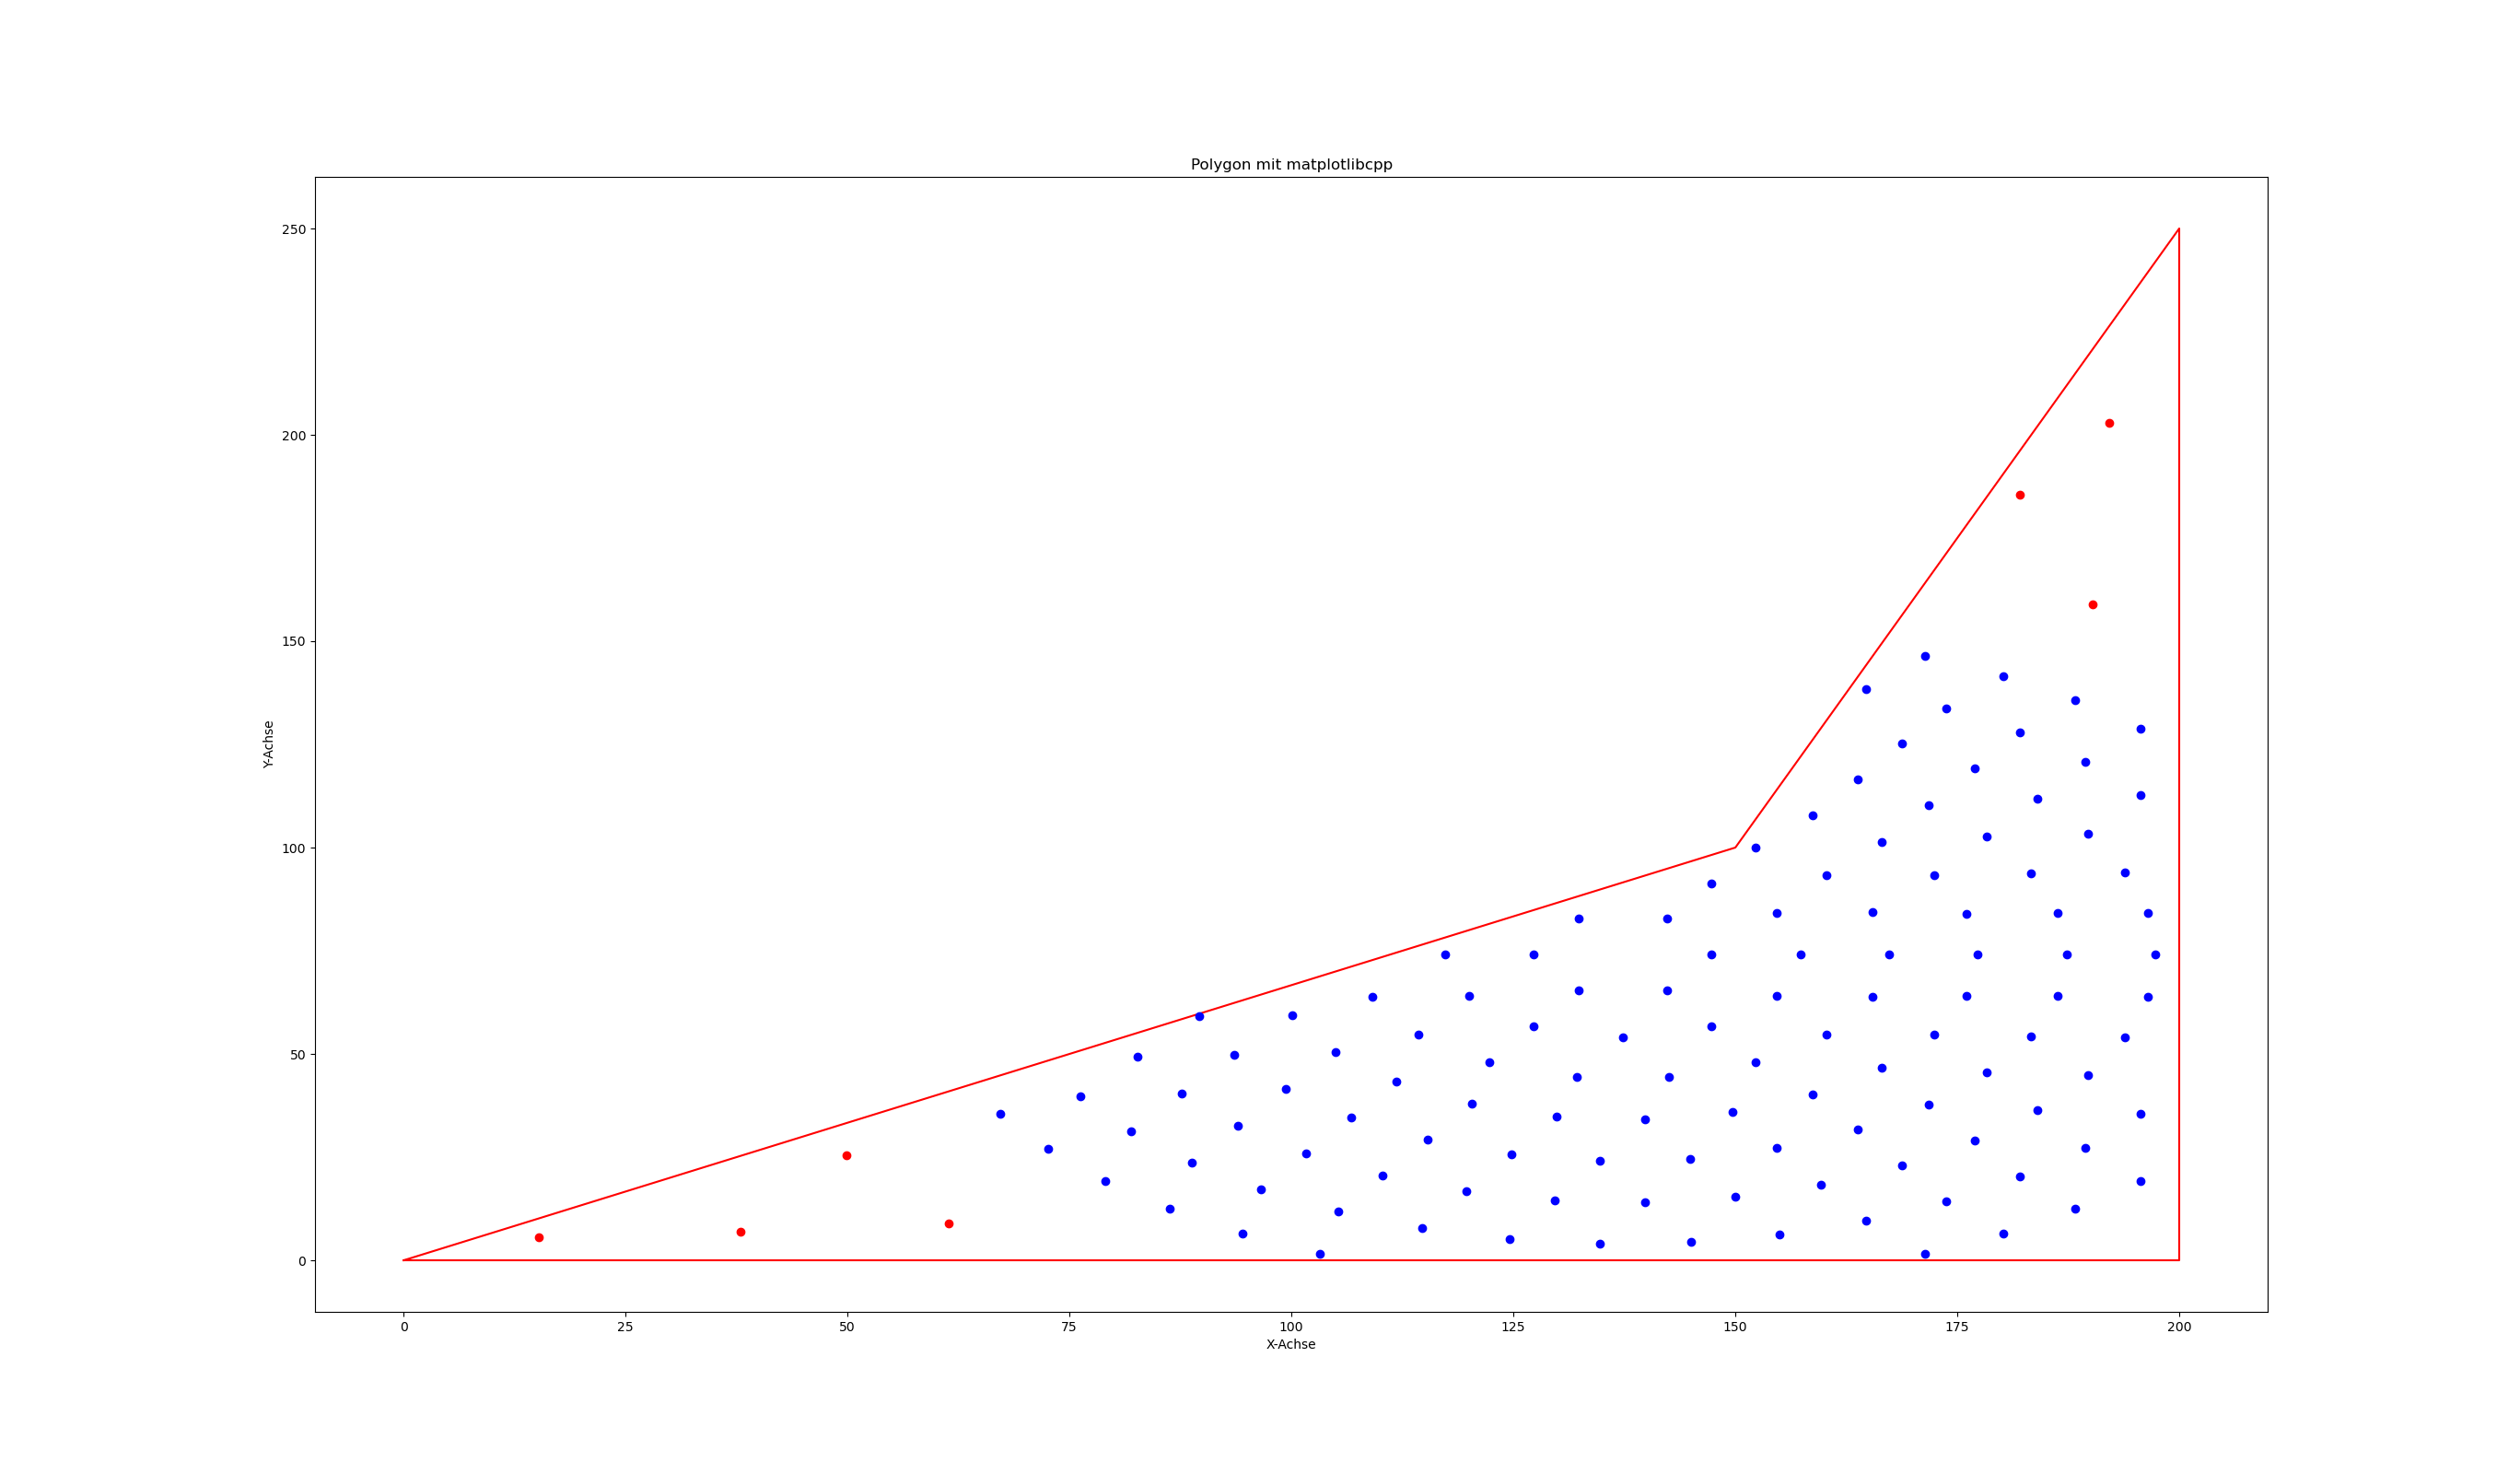
\includegraphics[width=1\textwidth]{Bilder/Figure_1.png}
    \caption{Polygon und Doerfer von siedler1.txt}
    \label{fig:example}
\end{figure}
\subsubsection{\textcolor{blue}{siedler2.txt}}
\begin{verbatim}
jetzt
jetzt
Gesundheitszentrum: (5|8.66025)
Doerfer innerhalb des Radiuses von dem Gesundheitszentrum: 
Das 1Dorf liegt bei den koordinaten: (15|8.66025)
Das 2Dorf liegt bei den koordinaten: (10|17.3205)
Das 3Dorf liegt bei den koordinaten: (2.66454e-15|17.3205)
Das 4Dorf liegt bei den koordinaten: (-5|8.66025)
Das 5Dorf liegt bei den koordinaten: (-3.55271e-15|1.77636e-15)
Das 6Dorf liegt bei den koordinaten: (10|0)
Das 7Dorf liegt bei den koordinaten: (22.3205|18.6603)
Das 8Dorf liegt bei den koordinaten: (5|28.6603)
Das 9Dorf liegt bei den koordinaten: (-12.3205|18.6603)
Das 10Dorf liegt bei den koordinaten: (-15|8.66025)
Das 11Dorf liegt bei den koordinaten: (-12.3205|-1.33975)
Das 12Dorf liegt bei den koordinaten: (-5|-8.66025)
Das 13Dorf liegt bei den koordinaten: (5|-11.3397)
Das 14Dorf liegt bei den koordinaten: (15|-8.66025)
Das 15Dorf liegt bei den koordinaten: (22.3205|-1.33975)
Das 16Dorf liegt bei den koordinaten: (35|8.66025)
Das 17Dorf liegt bei den koordinaten: (27.9813|27.9439)
Das 18Dorf liegt bei den koordinaten: (-17.9813|27.9439)
Das 19Dorf liegt bei den koordinaten: (-25|8.66025)
Das 20Dorf liegt bei den koordinaten: (-23.1908|-1.60035)
Das 21Dorf liegt bei den koordinaten: (-17.9813|-10.6234)
Das 22Dorf liegt bei den koordinaten: (-10|-17.3205)
Das 23Dorf liegt bei den koordinaten: (-0.209445|-20.884)
Das 24Dorf liegt bei den koordinaten: (10.2094|-20.884)
Das 25Dorf liegt bei den koordinaten: (20|-17.3205)
Das 26Dorf liegt bei den koordinaten: (27.9813|-10.6234)
Das 27Dorf liegt bei den koordinaten: (45|8.66025)
Das 28Dorf liegt bei den koordinaten: (34.1587|36.0421)
Das 29Dorf liegt bei den koordinaten: (-20.497|39.4808)
Das 30Dorf liegt bei den koordinaten: (-34.6846|13.6736)
Das 31Dorf liegt bei den koordinaten: (-32.1911|-6.06473)
Das 32Dorf liegt bei den koordinaten: (-20.497|-22.1603)
Das 33Dorf liegt bei den koordinaten: (-2.49525|-30.6312)
Das 34Dorf liegt bei den koordinaten: (17.3607|-29.382)
Das 35Dorf liegt bei den koordinaten: (34.1587|-18.7216)
Das 36Dorf liegt bei den koordinaten: (39.4483|44.8999)
Das 37Dorf liegt bei den koordinaten: (2.46754|58.5961)
Das 38Dorf liegt bei den koordinaten: (-42.707|-6.3079)
Das 39Dorf liegt bei den koordinaten: (-25.6053|-30.8785)
Das 40Dorf liegt bei den koordinaten: (-7.53263|-39.7436)
Das 41Dorf liegt bei den koordinaten: (22.3653|-38.2274)
Das 42Dorf liegt bei den koordinaten: (46.0382|-19.9032)
Das 43Dorf liegt bei den koordinaten: (64.137|18.8003)
Das 44Dorf liegt bei den koordinaten: (-30.678|-39.5796)
Das 45Dorf liegt bei den koordinaten: (-2.62107|-50.8538)
Das 46Dorf liegt bei den koordinaten: (27.3714|-47.0131)
Das 47Dorf liegt bei den koordinaten: (57.3808|-20.6014)
Das 48Dorf liegt bei den koordinaten: (2.44346|78.6136)
Das 49Dorf liegt bei den koordinaten: (-63.3253|23.8804)
Das 50Dorf liegt bei den koordinaten: (-60.3811|-16.3459)
Das 51Dorf liegt bei den koordinaten: (-35.7301|-48.27)
Das 52Dorf liegt bei den koordinaten: (-69.3821|-20.7897)
Das 53Dorf liegt bei den koordinaten: (-0.0232416|-71.1819)
Restliche doerfer ausserhalb des Radiuses des gesundheitszentrums: 
Das 54Dorf liegt bei den koordinaten: (-0.0649169|-91.2114)
\end{verbatim}
\newpage
\begin{figure}[h]
    \centering
    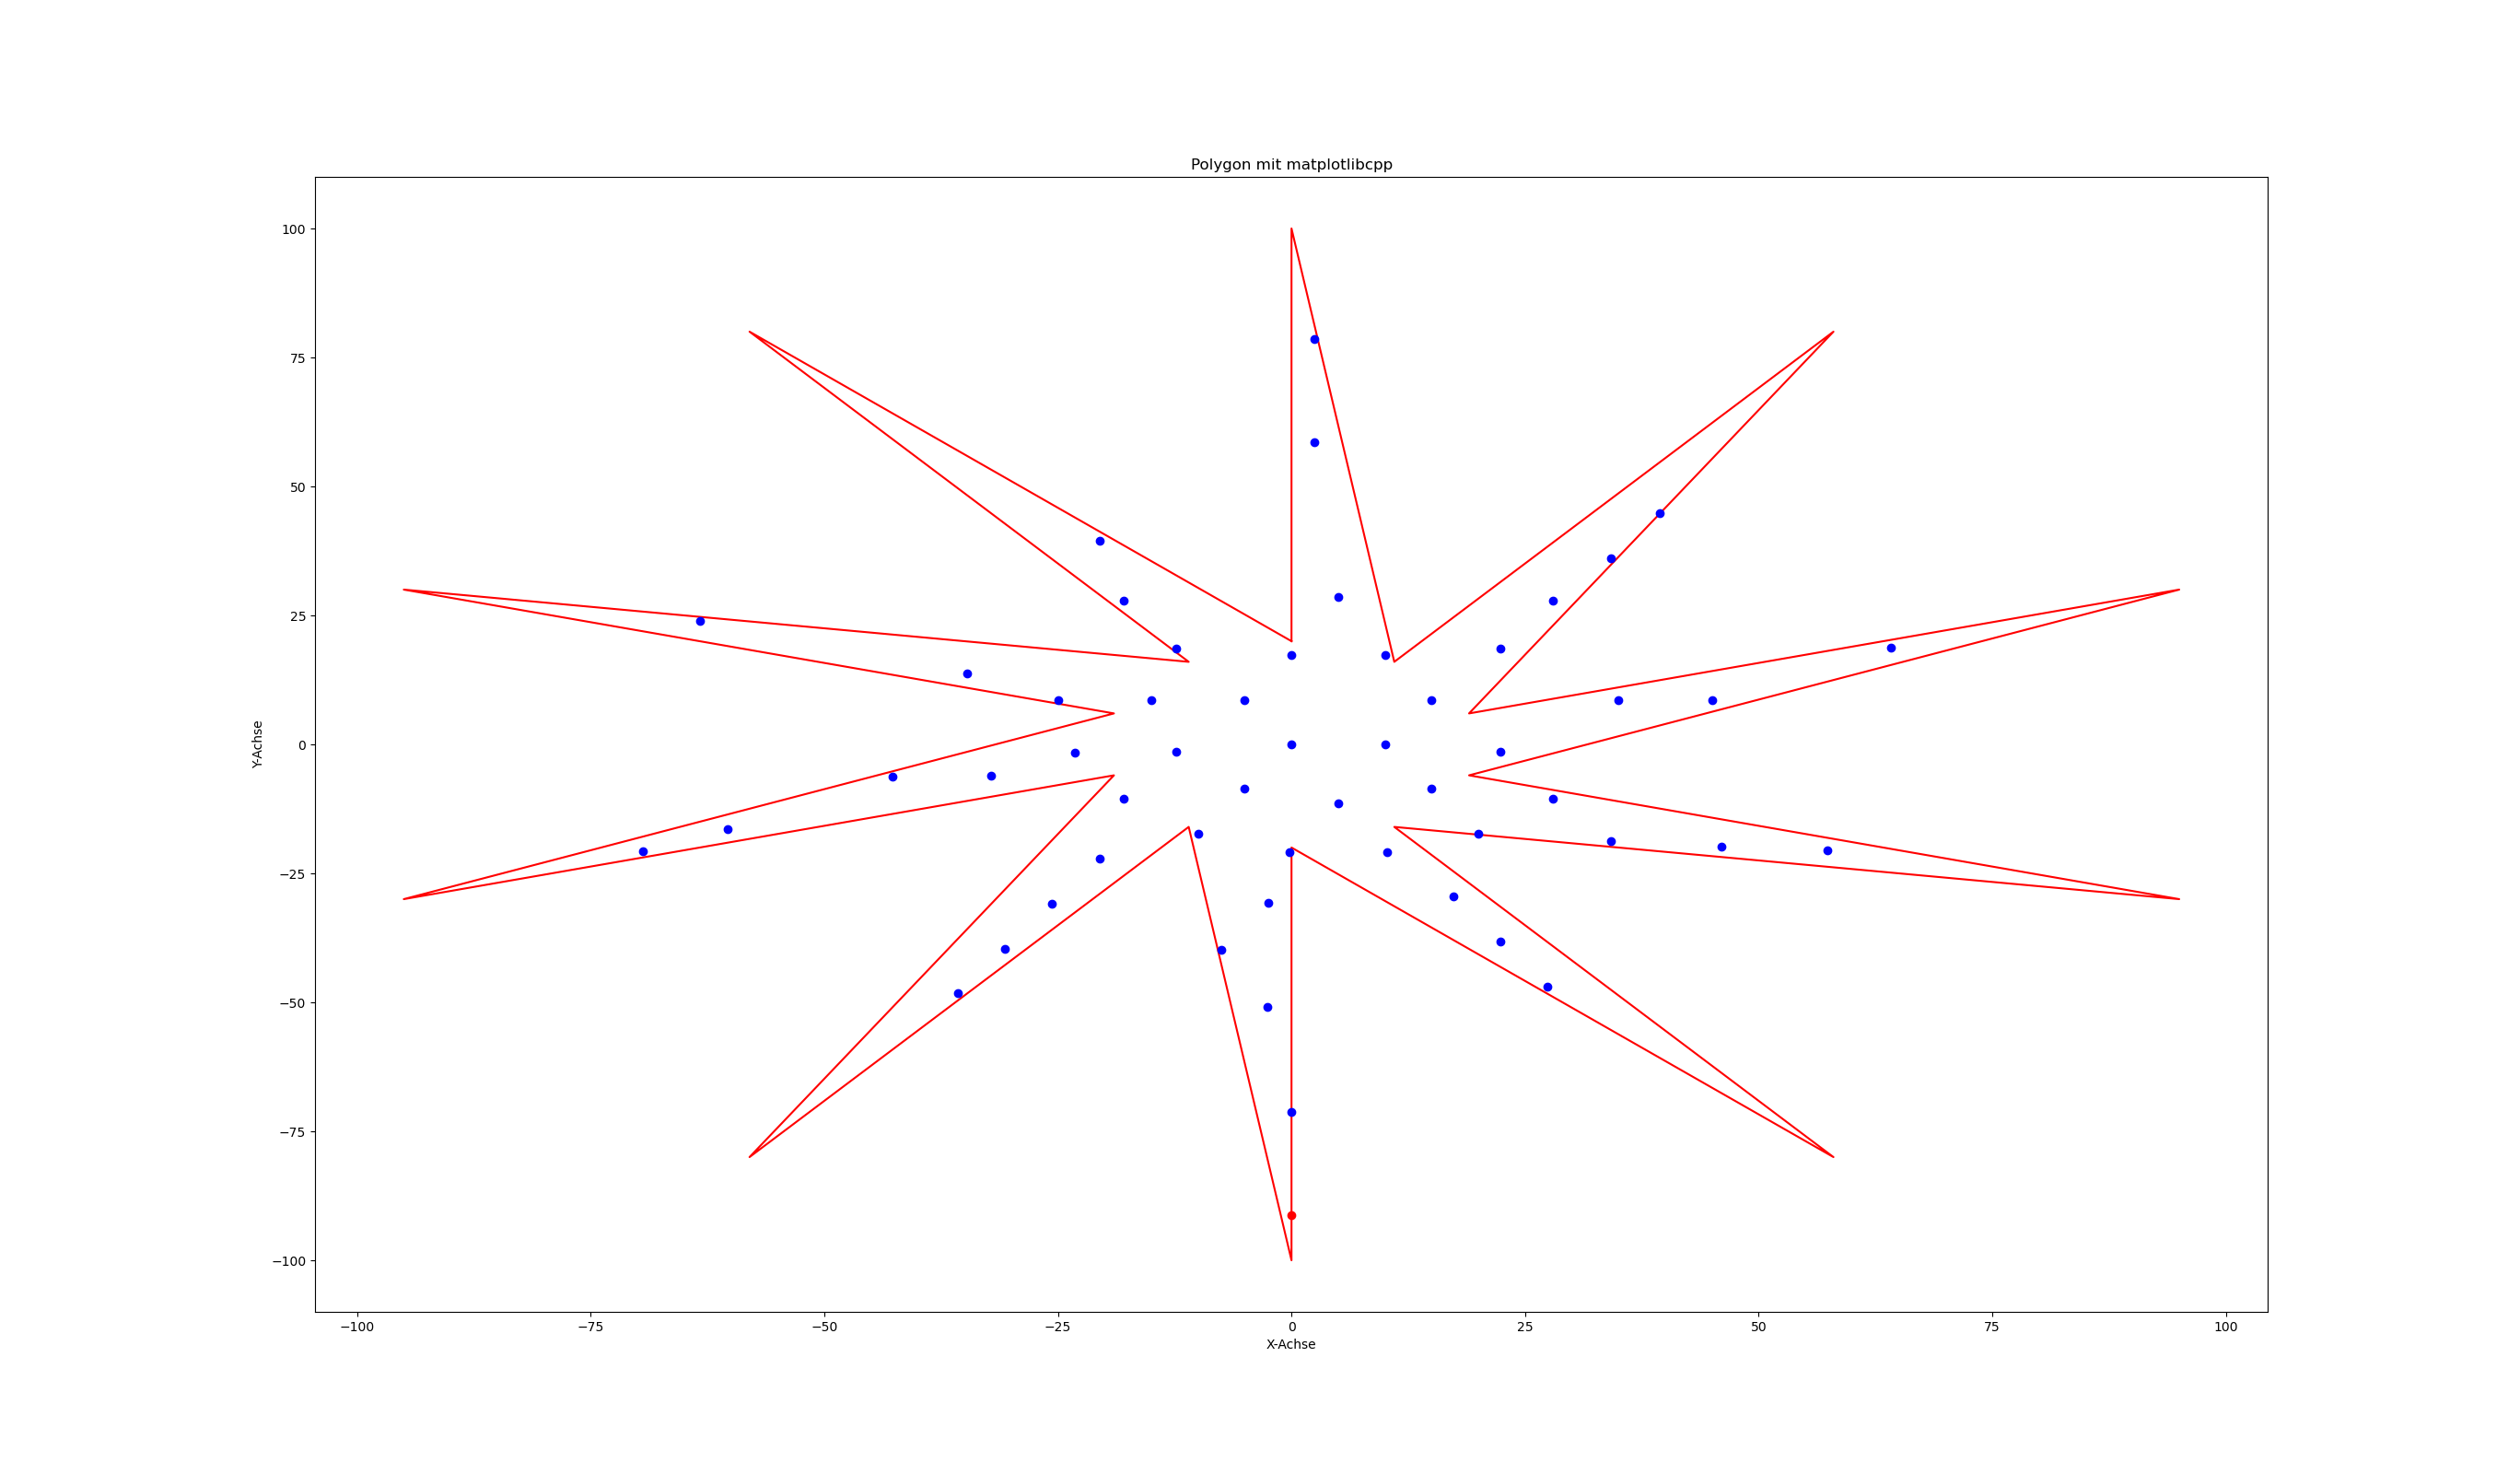
\includegraphics[width=1\textwidth]{Bilder/Figure_2.png}
    \caption{Polygon und Doerfer von siedler2.txt}
    \label{fig:example}
\end{figure}
\subsubsection{\textcolor{blue}{siedler3.txt}}
\begin{verbatim}
jetzt
jetzt
Gesundheitszentrum: (80|83.6603)
Doerfer innerhalb des Radiuses von dem Gesundheitszentrum: 
Das 1Dorf liegt bei den koordinaten: (90|83.6603)
Das 2Dorf liegt bei den koordinaten: (85|92.3205)
Das 3Dorf liegt bei den koordinaten: (75|92.3205)
Das 4Dorf liegt bei den koordinaten: (70|83.6603)
Das 5Dorf liegt bei den koordinaten: (75|75)
Das 6Dorf liegt bei den koordinaten: (85|75)
Das 7Dorf liegt bei den koordinaten: (100|83.6603)
Das 8Dorf liegt bei den koordinaten: (97.3205|93.6603)
Das 9Dorf liegt bei den koordinaten: (90|100.981)
Das 10Dorf liegt bei den koordinaten: (80|103.66)
Das 11Dorf liegt bei den koordinaten: (70|100.981)
Das 12Dorf liegt bei den koordinaten: (62.6795|93.6603)
Das 13Dorf liegt bei den koordinaten: (60|83.6603)
Das 14Dorf liegt bei den koordinaten: (62.6795|73.6603)
Das 15Dorf liegt bei den koordinaten: (70|66.3397)
Das 16Dorf liegt bei den koordinaten: (80|63.6603)
Das 17Dorf liegt bei den koordinaten: (90|66.3397)
Das 18Dorf liegt bei den koordinaten: (97.3205|73.6603)
Das 19Dorf liegt bei den koordinaten: (110|83.6603)
Das 20Dorf liegt bei den koordinaten: (108.191|93.9209)
Das 21Dorf liegt bei den koordinaten: (102.981|102.944)
Das 22Dorf liegt bei den koordinaten: (95|109.641)
Das 23Dorf liegt bei den koordinaten: (85.2094|113.204)
Das 24Dorf liegt bei den koordinaten: (74.7906|113.204)
Das 25Dorf liegt bei den koordinaten: (65|109.641)
Das 26Dorf liegt bei den koordinaten: (57.0187|102.944)
Das 27Dorf liegt bei den koordinaten: (51.8092|93.9209)
Das 28Dorf liegt bei den koordinaten: (50|83.6603)
Das 29Dorf liegt bei den koordinaten: (51.8092|73.3996)
Das 30Dorf liegt bei den koordinaten: (57.0187|64.3766)
Das 31Dorf liegt bei den koordinaten: (65|57.6795)
Das 32Dorf liegt bei den koordinaten: (74.7906|54.116)
Das 33Dorf liegt bei den koordinaten: (85.2094|54.116)
Das 34Dorf liegt bei den koordinaten: (95|57.6795)
Das 35Dorf liegt bei den koordinaten: (102.981|64.3766)
Das 36Dorf liegt bei den koordinaten: (108.191|73.3996)
Das 37Dorf liegt bei den koordinaten: (120|83.6603)
Das 38Dorf liegt bei den koordinaten: (118.743|93.6078)
Das 39Dorf liegt bei den koordinaten: (115.052|102.93)
Das 40Dorf liegt bei den koordinaten: (109.159|111.042)
Das 41Dorf liegt bei den koordinaten: (101.433|117.433)
Das 42Dorf liegt bei den koordinaten: (92.3607|121.703)
Das 43Dorf liegt bei den koordinaten: (82.5116|123.581)
Das 44Dorf liegt bei den koordinaten: (72.5047|122.952)
Das 45Dorf liegt bei den koordinaten: (62.9688|119.853)
Das 46Dorf liegt bei den koordinaten: (54.503|114.481)
Das 47Dorf liegt bei den koordinaten: (47.6393|107.172)
Das 48Dorf liegt bei den koordinaten: (42.8089|98.3852)
Das 49Dorf liegt bei den koordinaten: (40.3154|88.6736)
Das 50Dorf liegt bei den koordinaten: (40.3154|78.6469)
Das 51Dorf liegt bei den koordinaten: (42.8089|68.9353)
Das 52Dorf liegt bei den koordinaten: (47.6393|60.1488)
Das 53Dorf liegt bei den koordinaten: (54.503|52.8397)
Das 54Dorf liegt bei den koordinaten: (62.9688|47.4672)
Das 55Dorf liegt bei den koordinaten: (72.5047|44.3688)
Das 56Dorf liegt bei den koordinaten: (82.5116|43.7392)
Das 57Dorf liegt bei den koordinaten: (92.3607|45.618)
Das 58Dorf liegt bei den koordinaten: (101.433|49.8871)
Das 59Dorf liegt bei den koordinaten: (109.159|56.2784)
Das 60Dorf liegt bei den koordinaten: (115.052|64.3901)
Das 61Dorf liegt bei den koordinaten: (118.743|73.7127)
Das 62Dorf liegt bei den koordinaten: (130|83.6603)
Das 63Dorf liegt bei den koordinaten: (128.976|93.7252)
Das 64Dorf liegt bei den koordinaten: (125.948|103.378)
Das 65Dorf liegt bei den koordinaten: (121.038|112.224)
Das 66Dorf liegt bei den koordinaten: (114.448|119.9)
Das 67Dorf liegt bei den koordinaten: (106.448|126.092)
Das 68Dorf liegt bei den koordinaten: (97.3653|130.548)
Das 69Dorf liegt bei den koordinaten: (87.5714|133.084)
Das 70Dorf liegt bei den koordinaten: (77.4675|133.596)
Das 71Dorf liegt bei den koordinaten: (67.4674|132.064)
Das 72Dorf liegt bei den koordinaten: (57.9803|128.55)
Das 73Dorf liegt bei den koordinaten: (49.3947|123.199)
Das 74Dorf liegt bei den koordinaten: (42.0621|116.229)
Das 75Dorf liegt bei den koordinaten: (36.2827|107.925)
Das 76Dorf liegt bei den koordinaten: (32.293|98.6284)
Das 77Dorf liegt bei den koordinaten: (30.2565|88.7187)
Das 78Dorf liegt bei den koordinaten: (30.2565|78.6018)
Das 79Dorf liegt bei den koordinaten: (32.293|68.6921)
Das 80Dorf liegt bei den koordinaten: (36.2827|59.3952)
Das 81Dorf liegt bei den koordinaten: (42.0621|51.0916)
Das 82Dorf liegt bei den koordinaten: (49.3947|44.1215)
Das 83Dorf liegt bei den koordinaten: (57.9803|38.77)
Das 84Dorf liegt bei den koordinaten: (67.4674|35.2564)
Das 85Dorf liegt bei den koordinaten: (77.4675|33.7244)
Das 86Dorf liegt bei den koordinaten: (87.5714|34.2368)
Das 87Dorf liegt bei den koordinaten: (97.3653|36.7726)
Das 88Dorf liegt bei den koordinaten: (106.448|41.228)
Das 89Dorf liegt bei den koordinaten: (114.448|47.4206)
Das 90Dorf liegt bei den koordinaten: (121.038|55.0968)
Das 91Dorf liegt bei den koordinaten: (125.948|63.9425)
Das 92Dorf liegt bei den koordinaten: (128.976|73.5953)
Das 93Dorf liegt bei den koordinaten: (140|83.6603)
Das 94Dorf liegt bei den koordinaten: (139.137|93.8003)
Das 95Dorf liegt bei den koordinaten: (136.573|103.649)
Das 96Dorf liegt bei den koordinaten: (132.381|112.922)
Das 97Dorf liegt bei den koordinaten: (126.682|121.353)
Das 98Dorf liegt bei den koordinaten: (119.64|128.701)
Das 99Dorf liegt bei den koordinaten: (111.458|134.752)
Das 100Dorf liegt bei den koordinaten: (102.371|139.334)
Das 101Dorf liegt bei den koordinaten: (92.6408|142.314)
Das 102Dorf liegt bei den koordinaten: (82.5465|143.606)
Das 103Dorf liegt bei den koordinaten: (72.3789|143.174)
Das 104Dorf liegt bei den koordinaten: (62.4306|141.03)
Das 105Dorf liegt bei den koordinaten: (52.9878|137.236)
Das 106Dorf liegt bei den koordinaten: (44.322|131.9)
Das 107Dorf liegt bei den koordinaten: (36.6826|125.177)
Das 108Dorf liegt bei den koordinaten: (30.2894|117.259)
Das 109Dorf liegt bei den koordinaten: (25.3263|108.374)
Das 110Dorf liegt bei den koordinaten: (21.936|98.7789)
Das 111Dorf liegt bei den koordinaten: (20.2162|88.7486)
Das 112Dorf liegt bei den koordinaten: (20.2162|78.5719)
Das 113Dorf liegt bei den koordinaten: (21.936|68.5416)
Das 114Dorf liegt bei den koordinaten: (25.3263|58.9462)
Das 115Dorf liegt bei den koordinaten: (30.2894|50.0618)
Das 116Dorf liegt bei den koordinaten: (36.6826|42.1439)
Das 117Dorf liegt bei den koordinaten: (44.322|35.4204)
Das 118Dorf liegt bei den koordinaten: (52.9878|30.0847)
Das 119Dorf liegt bei den koordinaten: (62.4306|26.2902)
Das 120Dorf liegt bei den koordinaten: (72.3789|24.1462)
Das 121Dorf liegt bei den koordinaten: (82.5465|23.7143)
Das 122Dorf liegt bei den koordinaten: (92.6408|25.0069)
Das 123Dorf liegt bei den koordinaten: (102.371|27.9869)
Das 124Dorf liegt bei den koordinaten: (111.458|32.5685)
Das 125Dorf liegt bei den koordinaten: (119.64|38.6199)
Das 126Dorf liegt bei den koordinaten: (126.682|45.9671)
Das 127Dorf liegt bei den koordinaten: (132.381|54.3986)
Das 128Dorf liegt bei den koordinaten: (136.573|63.6719)
Das 129Dorf liegt bei den koordinaten: (139.137|73.5202)
Das 130Dorf liegt bei den koordinaten: (149.254|93.8523)
Das 131Dorf liegt bei den koordinaten: (147.032|103.827)
Das 132Dorf liegt bei den koordinaten: (143.381|113.372)
Das 133Dorf liegt bei den koordinaten: (138.38|122.284)
Das 134Dorf liegt bei den koordinaten: (132.134|130.373)
Das 135Dorf liegt bei den koordinaten: (124.777|137.466)
Das 136Dorf liegt bei den koordinaten: (116.466|143.412)
Das 137Dorf liegt bei den koordinaten: (107.377|148.084)
Das 138Dorf liegt bei den koordinaten: (57.3984|149.911)
Das 139Dorf liegt bei den koordinaten: (47.993|145.914)
Das 140Dorf liegt bei den koordinaten: (39.2699|140.591)
Das 141Dorf liegt bei den koordinaten: (31.4148|134.053)
Das 142Dorf liegt bei den koordinaten: (24.5952|126.442)
Das 143Dorf liegt bei den koordinaten: (18.9565|117.92)
Das 144Dorf liegt bei den koordinaten: (14.6189|108.666)
Das 145Dorf liegt bei den koordinaten: (11.6747|98.8804)
Das 146Dorf liegt bei den koordinaten: (10.1867|88.7699)
Das 147Dorf liegt bei den koordinaten: (10.1867|78.5506)
Das 148Dorf liegt bei den koordinaten: (11.6747|68.4401)
Das 149Dorf liegt bei den koordinaten: (14.6189|58.6541)
Das 150Dorf liegt bei den koordinaten: (18.9565|49.401)
Das 151Dorf liegt bei den koordinaten: (24.5952|40.8781)
Das 152Dorf liegt bei den koordinaten: (31.4148|33.267)
Das 153Dorf liegt bei den koordinaten: (39.2699|26.73)
Das 154Dorf liegt bei den koordinaten: (47.993|21.4063)
Das 155Dorf liegt bei den koordinaten: (57.3984|17.4095)
Das 156Dorf liegt bei den koordinaten: (67.2854|14.8247)
Das 157Dorf liegt bei den koordinaten: (77.4435|13.707)
Das 158Dorf liegt bei den koordinaten: (87.656|14.0802)
Das 159Dorf liegt bei den koordinaten: (97.7053|15.9364)
Das 160Dorf liegt bei den koordinaten: (107.377|19.236)
Das 161Dorf liegt bei den koordinaten: (116.466|23.9087)
Das 162Dorf liegt bei den koordinaten: (124.777|29.855)
Das 163Dorf liegt bei den koordinaten: (132.134|36.9479)
Das 164Dorf liegt bei den koordinaten: (138.38|45.0365)
Das 165Dorf liegt bei den koordinaten: (143.381|53.9483)
Das 166Dorf liegt bei den koordinaten: (147.032|63.4933)
Das 167Dorf liegt bei den koordinaten: (149.254|73.4682)
Das 168Dorf liegt bei den koordinaten: (144.721|130.683)
Das 169Dorf liegt bei den koordinaten: (138.317|138.424)
Das 170Dorf liegt bei den koordinaten: (130.994|145.301)
Das 171Dorf liegt bei den koordinaten: (29.0061|145.301)
Das 172Dorf liegt bei den koordinaten: (21.6825|138.424)
Das 173Dorf liegt bei den koordinaten: (15.2786|130.683)
Das 174Dorf liegt bei den koordinaten: (9.89547|122.201)
Das 175Dorf liegt bei den koordinaten: (5.61788|113.11)
Das 176Dorf liegt bei den koordinaten: (2.51335|103.555)
Das 177Dorf liegt bei den koordinaten: (0.630824|93.6869)
Das 178Dorf liegt bei den koordinaten: (0|83.6603)
Das 179Dorf liegt bei den koordinaten: (0.630824|73.6336)
Das 180Dorf liegt bei den koordinaten: (2.51335|63.7651)
Das 181Dorf liegt bei den koordinaten: (5.61788|54.2103)
Das 182Dorf liegt bei den koordinaten: (9.89547|45.12)
Das 183Dorf liegt bei den koordinaten: (15.2786|36.6374)
Das 184Dorf liegt bei den koordinaten: (21.6825|28.8965)
Das 185Dorf liegt bei den koordinaten: (29.0061|22.0192)
Das 186Dorf liegt bei den koordinaten: (37.1339|16.114)
Das 187Dorf liegt bei den koordinaten: (45.9377|11.2741)
Das 188Dorf liegt bei den koordinaten: (55.2786|7.57573)
Das 189Dorf liegt bei den koordinaten: (65.0095|5.07727)
Das 190Dorf liegt bei den koordinaten: (74.9768|3.81812)
Das 191Dorf liegt bei den koordinaten: (85.0232|3.81812)
Das 192Dorf liegt bei den koordinaten: (94.9905|5.07727)
Das 193Dorf liegt bei den koordinaten: (104.721|7.57573)
Das 194Dorf liegt bei den koordinaten: (114.062|11.2741)
Das 195Dorf liegt bei den koordinaten: (122.866|16.114)
Das 196Dorf liegt bei den koordinaten: (130.994|22.0192)
Das 197Dorf liegt bei den koordinaten: (138.317|28.8965)
Das 198Dorf liegt bei den koordinaten: (144.721|36.6374)
Restliche doerfer ausserhalb des Radiuses des gesundheitszentrums: 
Das 199Dorf liegt bei den koordinaten: (4.12419|148.798)
Das 200Dorf liegt bei den koordinaten: (4.12419|18.523)
Das 201Dorf liegt bei den koordinaten: (18.7894|4.58268)
Das 202Dorf liegt bei den koordinaten: (148.897|11.181)

\end{verbatim}
\newpage
\begin{figure}[h]
    \centering
    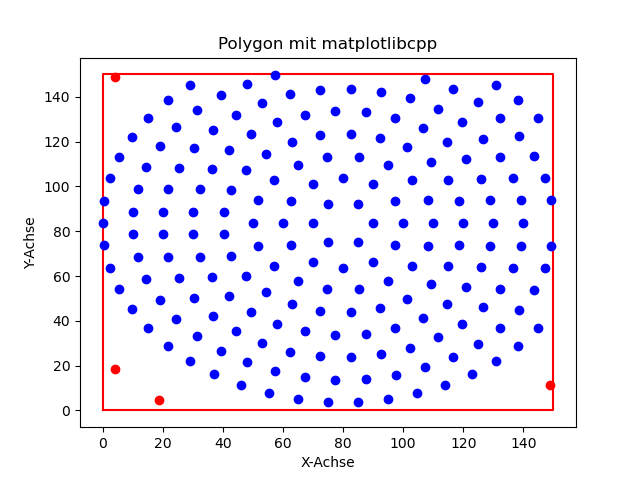
\includegraphics[width=1\textwidth]{Bilder/Figure_3.png}
    \caption{Polygon und Doerfer von siedler3.txt}
    \label{fig:example}
\end{figure}
\subsubsection{\textcolor{blue}{siedler4.txt}}
\begin{verbatim}
jetzt
jetzt
Gesundheitszentrum: (100.897|31.7372)
Doerfer innerhalb des Radiuses von dem Gesundheitszentrum: 
Das 1Dorf liegt bei den koordinaten: (110.897|31.7372)
Das 2Dorf liegt bei den koordinaten: (105.897|40.3974)
Das 3Dorf liegt bei den koordinaten: (90.8974|31.7372)
Das 4Dorf liegt bei den koordinaten: (95.8974|23.0769)
Das 5Dorf liegt bei den koordinaten: (105.897|23.0769)
Das 6Dorf liegt bei den koordinaten: (120.897|31.7372)
Das 7Dorf liegt bei den koordinaten: (110.897|49.0577)
Das 8Dorf liegt bei den koordinaten: (100.897|51.7372)
Das 9Dorf liegt bei den koordinaten: (90.8974|49.0577)
Das 10Dorf liegt bei den koordinaten: (83.5769|41.7372)
Das 11Dorf liegt bei den koordinaten: (80.8974|31.7372)
Das 12Dorf liegt bei den koordinaten: (83.5769|21.7372)
Das 13Dorf liegt bei den koordinaten: (90.8974|14.4167)
Das 14Dorf liegt bei den koordinaten: (100.897|11.7372)
Das 15Dorf liegt bei den koordinaten: (110.897|14.4167)
Das 16Dorf liegt bei den koordinaten: (118.218|21.7372)
Das 17Dorf liegt bei den koordinaten: (130.897|31.7372)
Das 18Dorf liegt bei den koordinaten: (129.088|41.9978)
Das 19Dorf liegt bei den koordinaten: (123.879|51.0208)
Das 20Dorf liegt bei den koordinaten: (106.107|61.2814)
Das 21Dorf liegt bei den koordinaten: (85.8974|57.7179)
Das 22Dorf liegt bei den koordinaten: (72.7067|41.9978)
Das 23Dorf liegt bei den koordinaten: (70.8974|31.7372)
Das 24Dorf liegt bei den koordinaten: (72.7067|21.4766)
Das 25Dorf liegt bei den koordinaten: (77.9161|12.4535)
Das 26Dorf liegt bei den koordinaten: (85.8974|5.75642)
Das 27Dorf liegt bei den koordinaten: (95.688|2.19294)
Das 28Dorf liegt bei den koordinaten: (106.107|2.19294)
Das 29Dorf liegt bei den koordinaten: (115.897|5.75642)
Das 30Dorf liegt bei den koordinaten: (123.879|12.4535)
Das 31Dorf liegt bei den koordinaten: (129.088|21.4766)
Das 32Dorf liegt bei den koordinaten: (140.897|31.7372)
Das 33Dorf liegt bei den koordinaten: (130.056|59.1191)
Das 34Dorf liegt bei den koordinaten: (122.331|65.5103)
Das 35Dorf liegt bei den koordinaten: (103.409|71.6582)
Das 36Dorf liegt bei den koordinaten: (83.8663|67.9303)
Das 37Dorf liegt bei den koordinaten: (68.5368|55.2486)
Das 38Dorf liegt bei den koordinaten: (63.7064|46.4622)
Das 39Dorf liegt bei den koordinaten: (61.2128|36.7505)
Das 40Dorf liegt bei den koordinaten: (61.2128|26.7238)
Das 41Dorf liegt bei den koordinaten: (63.7064|17.0122)
Das 42Dorf liegt bei den koordinaten: (68.5368|8.22577)
Das 43Dorf liegt bei den koordinaten: (75.4005|0.916647)
Das 44Dorf liegt bei den koordinaten: (83.8663|-4.4559)
Das 45Dorf liegt bei den koordinaten: (93.4022|-7.55431)
Das 46Dorf liegt bei den koordinaten: (103.409|-8.18389)
Das 47Dorf liegt bei den koordinaten: (113.258|-6.30508)
Das 48Dorf liegt bei den koordinaten: (122.331|-2.03594)
Das 49Dorf liegt bei den koordinaten: (130.056|4.35529)
Das 50Dorf liegt bei den koordinaten: (135.95|12.467)
Das 51Dorf liegt bei den koordinaten: (150.897|31.7372)
Das 52Dorf liegt bei den koordinaten: (149.874|41.8021)
Das 53Dorf liegt bei den koordinaten: (146.845|51.455)
Das 54Dorf liegt bei den koordinaten: (141.936|60.3006)
Das 55Dorf liegt bei den koordinaten: (62.9595|64.3058)
Das 56Dorf liegt bei den koordinaten: (53.1905|46.7053)
Das 57Dorf liegt bei den koordinaten: (51.154|36.7956)
Das 58Dorf liegt bei den koordinaten: (51.154|26.6788)
Das 59Dorf liegt bei den koordinaten: (53.1905|16.769)
Das 60Dorf liegt bei den koordinaten: (57.1801|7.47208)
Das 61Dorf liegt bei den koordinaten: (62.9595|-0.831447)
Das 62Dorf liegt bei den koordinaten: (70.2921|-7.80161)
Das 63Dorf liegt bei den koordinaten: (78.8777|-13.153)
Das 64Dorf liegt bei den koordinaten: (88.3648|-16.6667)
Das 65Dorf liegt bei den koordinaten: (98.365|-18.1986)
Das 66Dorf liegt bei den koordinaten: (108.469|-17.6862)
Das 67Dorf liegt bei den koordinaten: (118.263|-15.1504)
Das 68Dorf liegt bei den koordinaten: (127.346|-10.695)
Das 69Dorf liegt bei den koordinaten: (135.346|-4.50246)
Das 70Dorf liegt bei den koordinaten: (141.936|3.17377)
Das 71Dorf liegt bei den koordinaten: (146.845|12.0194)
Das 72Dorf liegt bei den koordinaten: (149.874|21.6723)
Das 73Dorf liegt bei den koordinaten: (160.897|31.7372)
Das 74Dorf liegt bei den koordinaten: (160.034|41.8772)
Das 75Dorf liegt bei den koordinaten: (147.58|69.4304)
Das 76Dorf liegt bei den koordinaten: (140.538|76.7775)
Das 77Dorf liegt bei den koordinaten: (46.2237|56.4513)
Das 78Dorf liegt bei den koordinaten: (42.8335|46.8559)
Das 79Dorf liegt bei den koordinaten: (41.1136|36.8255)
Das 80Dorf liegt bei den koordinaten: (41.1136|26.6488)
Das 81Dorf liegt bei den koordinaten: (42.8335|16.6185)
Das 82Dorf liegt bei den koordinaten: (46.2237|7.0231)
Das 83Dorf liegt bei den koordinaten: (51.1869|-1.86131)
Das 84Dorf liegt bei den koordinaten: (57.5801|-9.77916)
Das 85Dorf liegt bei den koordinaten: (65.2194|-16.5027)
Das 86Dorf liegt bei den koordinaten: (132.356|-19.3546)
Das 87Dorf liegt bei den koordinaten: (140.538|-13.3032)
Das 88Dorf liegt bei den koordinaten: (147.58|-5.95602)
Das 89Dorf liegt bei den koordinaten: (153.278|2.47548)
Das 90Dorf liegt bei den koordinaten: (157.47|11.7488)
Das 91Dorf liegt bei den koordinaten: (160.034|21.5971)
Das 92Dorf liegt bei den koordinaten: (170.897|31.7372)
Das 93Dorf liegt bei den koordinaten: (170.151|41.9293)
Das 94Dorf liegt bei den koordinaten: (167.929|51.9041)
Das 95Dorf liegt bei den koordinaten: (164.279|61.4491)
Das 96Dorf liegt bei den koordinaten: (60.1673|88.6675)
Das 97Dorf liegt bei den koordinaten: (45.4927|74.5193)
Das 98Dorf liegt bei den koordinaten: (32.5721|46.9573)
Das 99Dorf liegt bei den koordinaten: (31.0842|36.8468)
Das 100Dorf liegt bei den koordinaten: (31.0842|26.6275)
Das 101Dorf liegt bei den koordinaten: (32.5721|16.5171)
Das 102Dorf liegt bei den koordinaten: (35.5163|6.73101)
Das 103Dorf liegt bei den koordinaten: (39.854|-2.52207)
Das 104Dorf liegt bei den koordinaten: (45.4927|-11.045)
Das 105Dorf liegt bei den koordinaten: (52.3122|-18.6561)
Das 106Dorf liegt bei den koordinaten: (153.031|-14.9751)
Das 107Dorf liegt bei den koordinaten: (159.277|-6.88656)
Das 108Dorf liegt bei den koordinaten: (164.279|2.02521)
Das 109Dorf liegt bei den koordinaten: (167.929|11.5702)
Das 110Dorf liegt bei den koordinaten: (170.151|21.5451)
Das 111Dorf liegt bei den koordinaten: (180.897|31.7372)
Das 112Dorf liegt bei den koordinaten: (180.267|41.7638)
Das 113Dorf liegt bei den koordinaten: (42.5799|86.5009)
Das 114Dorf liegt bei den koordinaten: (26.5153|61.1871)
Das 115Dorf liegt bei den koordinaten: (23.4108|51.6324)
Das 116Dorf liegt bei den koordinaten: (21.5283|41.7638)
Das 117Dorf liegt bei den koordinaten: (20.8974|31.7372)
Das 118Dorf liegt bei den koordinaten: (21.5283|21.7105)
Das 119Dorf liegt bei den koordinaten: (23.4108|11.842)
Das 120Dorf liegt bei den koordinaten: (26.5153|2.28721)
Das 121Dorf liegt bei den koordinaten: (30.7929|-6.80312)
Das 122Dorf liegt bei den koordinaten: (36.1761|-15.2856)
Das 123Dorf liegt bei den koordinaten: (165.619|-15.2856)
Das 124Dorf liegt bei den koordinaten: (171.002|-6.80312)
Das 125Dorf liegt bei den koordinaten: (175.28|2.28721)
Das 126Dorf liegt bei den koordinaten: (178.384|11.842)
Das 127Dorf liegt bei den koordinaten: (180.267|21.7105)
Restliche doerfer ausserhalb des Radiuses des gesundheitszentrums: 
Das 128Dorf liegt bei den koordinaten: (5.48351|61.6735)
Das 129Dorf liegt bei den koordinaten: (1.4105|41.854)
Das 130Dorf liegt bei den koordinaten: (1.4105|21.6203)
Das 131Dorf liegt bei den koordinaten: (5.48351|1.80086)
Das 132Dorf liegt bei den koordinaten: (13.4628|-16.793)
Das 133Dorf liegt bei den koordinaten: (192.793|-7.69841)

\end{verbatim}
\newpage
\begin{figure}[h]
    \centering
    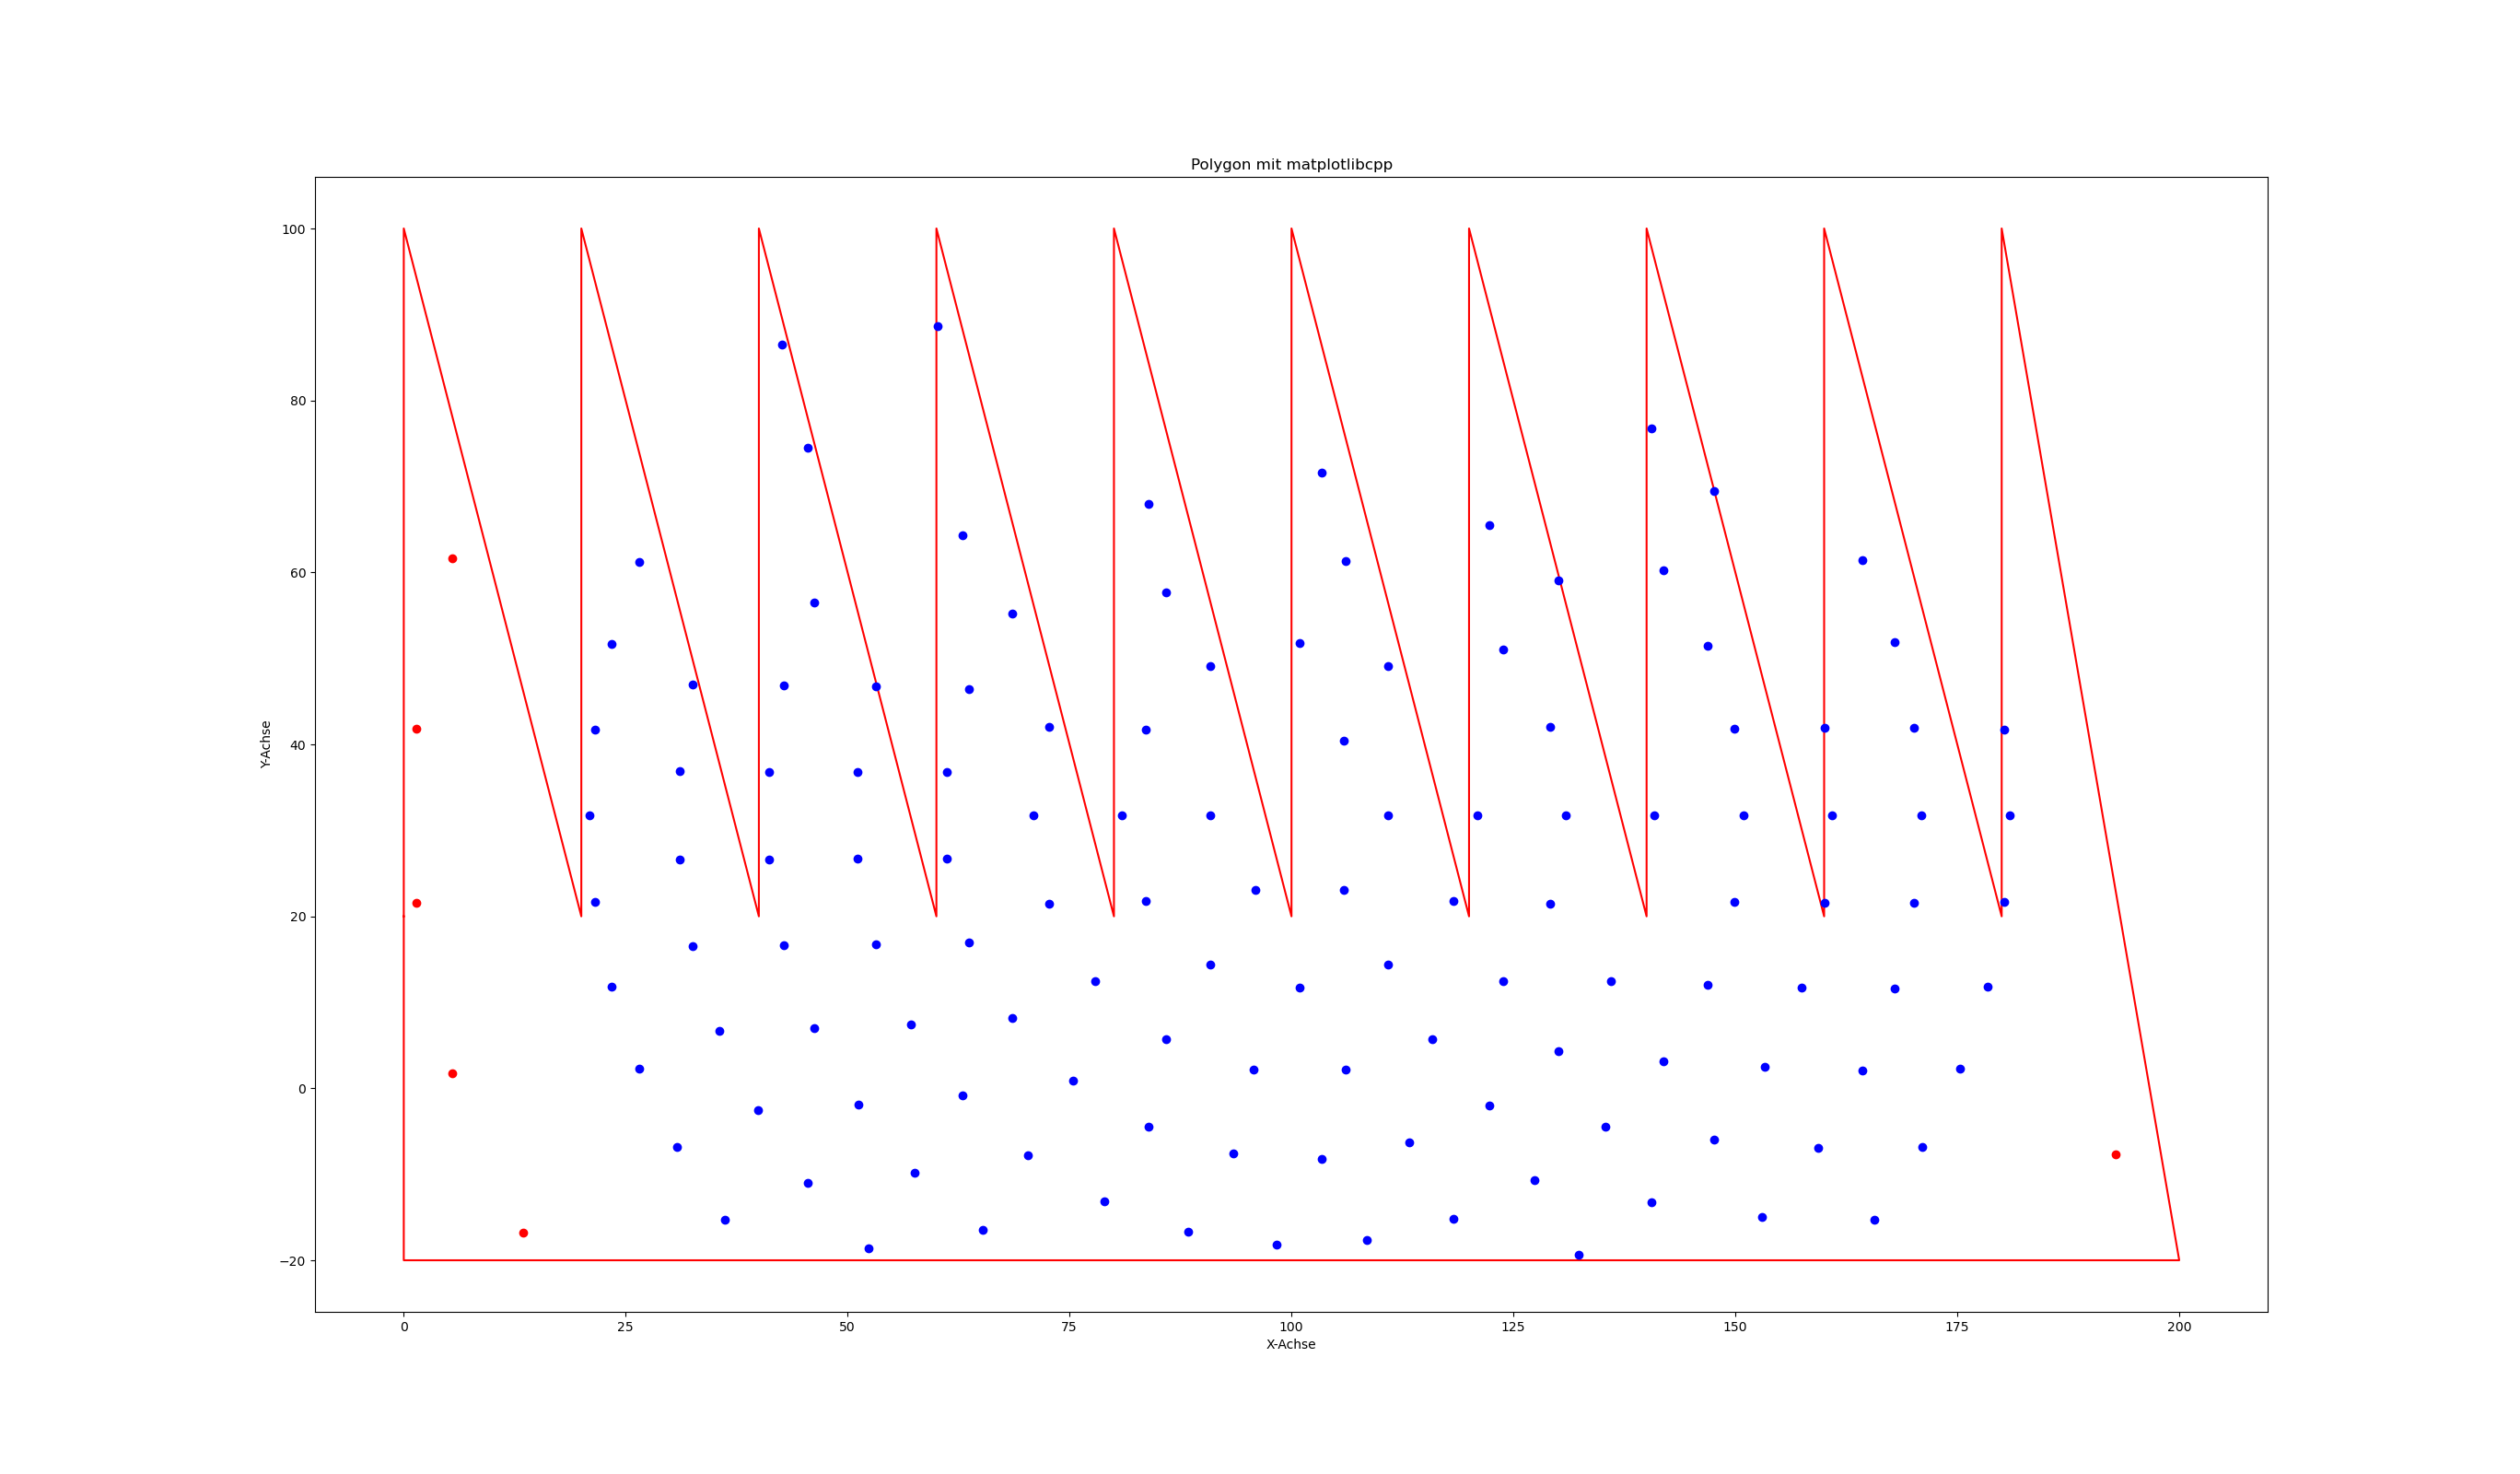
\includegraphics[width=1\textwidth]{Bilder/Figure_4.png}
    \caption{Polygon und Doerfer von siedler4.txt}
    \label{fig:example}
\end{figure}
\subsubsection{\textcolor{blue}{sielder5.txt}}
\begin{verbatim}
jetzt
jetzt
Gesundheitszentrum: (110|58.7149)
Doerfer innerhalb des Radiuses von dem Gesundheitszentrum: 
Das 1Dorf liegt bei den koordinaten: (120|58.7149)
Das 2Dorf liegt bei den koordinaten: (115|67.3752)
Das 3Dorf liegt bei den koordinaten: (115|50.0547)
Das 4Dorf liegt bei den koordinaten: (130|58.7149)
Das 5Dorf liegt bei den koordinaten: (127.321|68.7149)
Das 6Dorf liegt bei den koordinaten: (120|76.0354)
Das 7Dorf liegt bei den koordinaten: (110|78.7149)
Das 8Dorf liegt bei den koordinaten: (92.6795|68.7149)
Das 9Dorf liegt bei den koordinaten: (90|58.7149)
Das 10Dorf liegt bei den koordinaten: (92.6795|48.7149)
Das 11Dorf liegt bei den koordinaten: (100|41.3944)
Das 12Dorf liegt bei den koordinaten: (110|38.7149)
Das 13Dorf liegt bei den koordinaten: (120|41.3944)
Das 14Dorf liegt bei den koordinaten: (127.321|48.7149)
Das 15Dorf liegt bei den koordinaten: (140|58.7149)
Das 16Dorf liegt bei den koordinaten: (138.191|68.9755)
Das 17Dorf liegt bei den koordinaten: (132.981|77.9986)
Das 18Dorf liegt bei den koordinaten: (125|84.6957)
Das 19Dorf liegt bei den koordinaten: (115.209|88.2592)
Das 20Dorf liegt bei den koordinaten: (95|84.6957)
Das 21Dorf liegt bei den koordinaten: (87.0187|77.9986)
Das 22Dorf liegt bei den koordinaten: (81.8092|68.9755)
Das 23Dorf liegt bei den koordinaten: (80|58.7149)
Das 24Dorf liegt bei den koordinaten: (81.8092|48.4543)
Das 25Dorf liegt bei den koordinaten: (87.0187|39.4313)
Das 26Dorf liegt bei den koordinaten: (95|32.7342)
Das 27Dorf liegt bei den koordinaten: (115.209|29.1707)
Das 28Dorf liegt bei den koordinaten: (125|32.7342)
Das 29Dorf liegt bei den koordinaten: (132.981|39.4313)
Das 30Dorf liegt bei den koordinaten: (138.191|48.4543)
Das 31Dorf liegt bei den koordinaten: (150|58.7149)
Das 32Dorf liegt bei den koordinaten: (148.743|68.6625)
Das 33Dorf liegt bei den koordinaten: (145.052|77.9851)
Das 34Dorf liegt bei den koordinaten: (139.159|86.0968)
Das 35Dorf liegt bei den koordinaten: (131.433|92.488)
Das 36Dorf liegt bei den koordinaten: (122.361|96.7572)
Das 37Dorf liegt bei den koordinaten: (112.512|98.636)
Das 38Dorf liegt bei den koordinaten: (102.505|98.0064)
Das 39Dorf liegt bei den koordinaten: (92.9688|94.908)
Das 40Dorf liegt bei den koordinaten: (84.503|89.5355)
Das 41Dorf liegt bei den koordinaten: (77.6393|82.2263)
Das 42Dorf liegt bei den koordinaten: (72.8089|73.4399)
Das 43Dorf liegt bei den koordinaten: (70.3154|63.7283)
Das 44Dorf liegt bei den koordinaten: (70.3154|53.7016)
Das 45Dorf liegt bei den koordinaten: (72.8089|43.9899)
Das 46Dorf liegt bei den koordinaten: (77.6393|35.2035)
Das 47Dorf liegt bei den koordinaten: (84.503|27.8944)
Das 48Dorf liegt bei den koordinaten: (92.9688|22.5218)
Das 49Dorf liegt bei den koordinaten: (102.505|19.4234)
Das 50Dorf liegt bei den koordinaten: (112.512|18.7939)
Das 51Dorf liegt bei den koordinaten: (122.361|20.6727)
Das 52Dorf liegt bei den koordinaten: (131.433|24.9418)
Das 53Dorf liegt bei den koordinaten: (139.159|31.333)
Das 54Dorf liegt bei den koordinaten: (145.052|39.4448)
Das 55Dorf liegt bei den koordinaten: (148.743|48.7673)
Das 56Dorf liegt bei den koordinaten: (160|58.7149)
Das 57Dorf liegt bei den koordinaten: (158.976|68.7799)
Das 58Dorf liegt bei den koordinaten: (155.948|78.4327)
Das 59Dorf liegt bei den koordinaten: (151.038|87.2783)
Das 60Dorf liegt bei den koordinaten: (144.448|94.9546)
Das 61Dorf liegt bei den koordinaten: (79.3947|98.2537)
Das 62Dorf liegt bei den koordinaten: (72.0621|91.2836)
Das 63Dorf liegt bei den koordinaten: (66.2827|82.98)
Das 64Dorf liegt bei den koordinaten: (62.293|73.6831)
Das 65Dorf liegt bei den koordinaten: (60.2565|63.7733)
Das 66Dorf liegt bei den koordinaten: (60.2565|53.6565)
Das 67Dorf liegt bei den koordinaten: (62.293|43.7468)
Das 68Dorf liegt bei den koordinaten: (66.2827|34.4498)
Das 69Dorf liegt bei den koordinaten: (72.0621|26.1463)
Das 70Dorf liegt bei den koordinaten: (79.3947|19.1761)
Das 71Dorf liegt bei den koordinaten: (87.9803|13.8247)
Das 72Dorf liegt bei den koordinaten: (97.4674|10.3111)
Das 73Dorf liegt bei den koordinaten: (107.468|8.77911)
Das 74Dorf liegt bei den koordinaten: (117.571|9.29152)
Das 75Dorf liegt bei den koordinaten: (127.365|11.8273)
Das 76Dorf liegt bei den koordinaten: (136.448|16.2827)
Das 77Dorf liegt bei den koordinaten: (144.448|22.4753)
Das 78Dorf liegt bei den koordinaten: (151.038|30.1515)
Das 79Dorf liegt bei den koordinaten: (155.948|38.9971)
Das 80Dorf liegt bei den koordinaten: (158.976|48.65)
Das 81Dorf liegt bei den koordinaten: (170|58.7149)
Das 82Dorf liegt bei den koordinaten: (169.137|68.855)
Das 83Dorf liegt bei den koordinaten: (166.573|78.7033)
Das 84Dorf liegt bei den koordinaten: (162.381|87.9766)
Das 85Dorf liegt bei den koordinaten: (156.682|96.4081)
Das 86Dorf liegt bei den koordinaten: (60.2894|92.3134)
Das 87Dorf liegt bei den koordinaten: (55.3263|83.429)
Das 88Dorf liegt bei den koordinaten: (51.936|73.8336)
Das 89Dorf liegt bei den koordinaten: (50.2162|63.8033)
Das 90Dorf liegt bei den koordinaten: (50.2162|53.6266)
Das 91Dorf liegt bei den koordinaten: (51.936|43.5962)
Das 92Dorf liegt bei den koordinaten: (55.3263|34.0009)
Das 93Dorf liegt bei den koordinaten: (60.2894|25.1164)
Das 94Dorf liegt bei den koordinaten: (66.6826|17.1986)
Das 95Dorf liegt bei den koordinaten: (74.322|10.4751)
Das 96Dorf liegt bei den koordinaten: (82.9878|5.13938)
Das 97Dorf liegt bei den koordinaten: (92.4306|1.34493)
Das 98Dorf liegt bei den koordinaten: (122.641|0.0616177)
Das 99Dorf liegt bei den koordinaten: (132.371|3.04159)
Das 100Dorf liegt bei den koordinaten: (141.458|7.62318)
Das 101Dorf liegt bei den koordinaten: (149.64|13.6746)
Das 102Dorf liegt bei den koordinaten: (156.682|21.0217)
Das 103Dorf liegt bei den koordinaten: (162.381|29.4532)
Das 104Dorf liegt bei den koordinaten: (166.573|38.7265)
Das 105Dorf liegt bei den koordinaten: (169.137|48.5749)
Das 106Dorf liegt bei den koordinaten: (180|58.7149)
Das 107Dorf liegt bei den koordinaten: (179.254|68.907)
Das 108Dorf liegt bei den koordinaten: (177.032|78.8819)
Das 109Dorf liegt bei den koordinaten: (173.381|88.4269)
Das 110Dorf liegt bei den koordinaten: (168.38|97.3387)
Das 111Dorf liegt bei den koordinaten: (48.9565|92.9742)
Das 112Dorf liegt bei den koordinaten: (44.6189|83.7211)
Das 113Dorf liegt bei den koordinaten: (41.6747|73.935)
Das 114Dorf liegt bei den koordinaten: (40.1867|63.8246)
Das 115Dorf liegt bei den koordinaten: (40.1867|53.6053)
Das 116Dorf liegt bei den koordinaten: (41.6747|43.4948)
Das 117Dorf liegt bei den koordinaten: (44.6189|33.7088)
Das 118Dorf liegt bei den koordinaten: (48.9565|24.4557)
Das 119Dorf liegt bei den koordinaten: (54.5952|15.9328)
Das 120Dorf liegt bei den koordinaten: (61.4148|8.32169)
Das 121Dorf liegt bei den koordinaten: (69.2699|1.78465)
Das 122Dorf liegt bei den koordinaten: (154.777|4.90963)
Das 123Dorf liegt bei den koordinaten: (162.134|12.0026)
Das 124Dorf liegt bei den koordinaten: (168.38|20.0912)
Das 125Dorf liegt bei den koordinaten: (173.381|29.003)
Das 126Dorf liegt bei den koordinaten: (177.032|38.548)
Das 127Dorf liegt bei den koordinaten: (179.254|48.5229)
Das 128Dorf liegt bei den koordinaten: (189.369|68.7416)
Das 129Dorf liegt bei den koordinaten: (187.487|78.6101)
Das 130Dorf liegt bei den koordinaten: (184.382|88.1649)
Das 131Dorf liegt bei den koordinaten: (180.105|97.2552)
Das 132Dorf liegt bei den koordinaten: (39.8955|97.2552)
Das 133Dorf liegt bei den koordinaten: (35.6179|88.1649)
Das 134Dorf liegt bei den koordinaten: (32.5133|78.6101)
Das 135Dorf liegt bei den koordinaten: (30.6308|68.7416)
Das 136Dorf liegt bei den koordinaten: (30|58.7149)
Das 137Dorf liegt bei den koordinaten: (30.6308|48.6883)
Das 138Dorf liegt bei den koordinaten: (32.5133|38.8197)
Das 139Dorf liegt bei den koordinaten: (35.6179|29.265)
Das 140Dorf liegt bei den koordinaten: (39.8955|20.1746)
Das 141Dorf liegt bei den koordinaten: (45.2786|11.6921)
Das 142Dorf liegt bei den koordinaten: (51.6825|3.95116)
Das 143Dorf liegt bei den koordinaten: (168.317|3.95116)
Das 144Dorf liegt bei den koordinaten: (174.721|11.6921)
Das 145Dorf liegt bei den koordinaten: (180.105|20.1746)
Das 146Dorf liegt bei den koordinaten: (184.382|29.265)
Das 147Dorf liegt bei den koordinaten: (187.487|38.8197)
Das 148Dorf liegt bei den koordinaten: (189.369|48.6883)
Restliche doerfer ausserhalb des Radiuses des gesundheitszentrums: 
Das 149Dorf liegt bei den koordinaten: (22.5653|10.1847)
\end{verbatim}
\newpage
\begin{figure}[h]
    \centering
    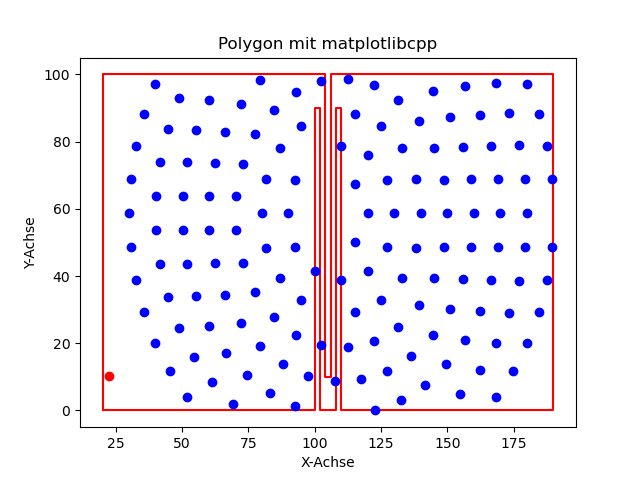
\includegraphics[width=1\textwidth]{Bilder/Figure_5.png}
    \caption{Polygon und Doerfer von siedler5.txt}
    \label{fig:example}
\end{figure}

\section{\textcolor{blue}{Quellcode}}
\subsection{\textcolor{blue}{Geometrie.h}}
\begin{verbatim}

#pragma once

#include <iostream>
#include <cmath>
#include <vector>
#include <sstream>
#include <fstream>

namespace Geometrie{

	// klasse point um ein punkt darzustellen
	class Point{
		private:
			double x,y;
		public:
		        Point() : x(0.0), y(0.0){}
			Point(double _x, double _y) : x(_x), y(_y){}

			// funktionen zum returnen der x und y koordinaten
			double getX() const {return x;}
			double getY() const  {return y;}

	};

	// klasse Polygon
	class Polygon{
		private:
			std::vector<Point> points;
		public:
			Polygon(){}

			std::vector<Point> getPoints() const{
				return points;
			}

			const Point& getPoint(int index) const{
				return points[index];
			}

			// Funktion um ein Punkt in das Polygon hinzuzufuegen
			void addPoint(double x, double y){
				points.push_back(Point(x,y));
			}

			void addPointsFromVector(const std::vector<Point>& vec) {
				points.insert(points.end(), vec.begin(), vec.end());
			}

			// Funktion zum Bestimmen des Schwerpunktes oder auch Centroid des Polygons
			Point centroid() const {
		         double cx = 0.0, cy = 0.0;
		         double area = 0.0;

		         for (int i = 0; i < points.size(); ++i) {
		             double xi = points[i].getX();
		             double yi = points[i].getY();

		             double xi1 = points[(i + 1) % points.size()].getX();
		             double yi1 = points[(i + 1) % points.size()].getY();

		             double common = xi * yi1 - xi1 * yi;
		             cx += (xi + xi1) * common;
		             cy += (yi + yi1) * common;
		             area += common;
		         }

		         area /= 2.0;
		         cx /= (6 * area);
		         cy /= (6 * area);

		         return Point(cx, cy);
			}

		// Funktion zum schauen ob der punkt innerhalb des polygons liegt oder nicht
			bool isInsidePolygon(const Point& p) const {
				int intersectioncount = 0;

				for(int i = 0; i < points.size(); ++i){
					double xi = points[i].getX();
					double yi = points[i].getY();
					double xi1 = points[(i + 1) % points.size()].getX();
					double yi1 = points[(i + 1) % points.size()].getY();

					if((yi > p.getY()) != (yi1 > p.getY()) && p.getX() < (xi1 - xi) *
					 (p.getY() - yi) / (yi1 - yi) + xi){
						intersectioncount++;
					}
				}

				return intersectioncount % 2 == 1;
			}
	 // Funktion zum einlesen des Polygons von der file .txt
	 void readPointsFromFile(const std::string& filename) {
		 std::ifstream file(filename);
		if (!file.is_open()) {
			std::cerr << "Fehler beim Öffnen der Datei: " << filename << std::endl;
				return;
		}

		std::string line;
		while (std::getline(file, line)) {
			std::stringstream ss(line);
				double x, y;
				if (ss >> x >> y) {
						addPoint(x, y);
				}
		}

		file.close();
}
	};
};
\end{verbatim}
\newpage
\subsection{\textcolor{blue}{main.cpp}}
\begin{verbatim}
#include <iostream>
#include <cmath>
#include <vector>

#include <Geometrie.h>
#include <matplotlibcpp.h>

namespace plt = matplotlibcpp;


// Funktion um die punkte eines umfangs Berechen
std::vector<Geometrie::Point> umfang_punkte_eins(const Geometrie::Polygon& polygon,
	Geometrie::Point centroid, int radius){
	std::vector<Geometrie::Point> umfang_Punkte;
	double umfang = 2 * M_PI * radius;
	int anzahl_punkte = static_cast<int>(umfang/20);

	for(int i = 0; i < anzahl_punkte; ++i){
		double winkel = (2*M_PI*i)/anzahl_punkte;
		double x = centroid.getX() + radius * std::cos(winkel);
		double y = centroid.getY() + radius * std::sin(winkel);
		if(polygon.isInsidePolygon(Geometrie::Point(x,y))){
			umfang_Punkte.push_back(Geometrie::Point(x, y));
		}
	}
	return umfang_Punkte;
}
// Funktion um die letzten punkte im polygon zu bestimmen
std::vector<Geometrie::Point> last_points(const Geometrie::Polygon& polygon,
	const Geometrie::Point& center_point) {
	int radius = 100;
	std::vector<Geometrie::Point> end_points;
	std::vector<Geometrie::Point> points = umfang_punkte_eins(polygon, center_point, radius);
	// endet wenn der kreis so gros ist das kein punkt mehr im polygon platziert werden kann
	while(points.size() > 0){
		end_points.insert(end_points.end(), points.begin(), points.end());
		radius += 20;
		points = umfang_punkte_eins(polygon, center_point, radius);
	}
	return end_points;
}

// Funktion zum berechen der Punkte auf dem Umkreis eines Kreises in 10 radius abstaenden bis 85
std::vector<Geometrie::Point> circle_Points(int distance, Geometrie::Point centroid_circle,
	const Geometrie::Polygon& polygon){
	std::vector<Geometrie::Point> umfang_Punkte;

	for(int radius = 10; radius <= 85; radius += 10){
		double umfang = 2 * M_PI * radius;
		int anzahl_punkte = static_cast<int>(umfang/distance);

		for(int i = 0; i < anzahl_punkte; ++i){
			double winkel = (2*M_PI*i)/anzahl_punkte;
			double x = centroid_circle.getX() + radius * std::cos(winkel);
			double y = centroid_circle.getY() + radius * std::sin(winkel);
			if(polygon.isInsidePolygon(Geometrie::Point(x,y))){
				umfang_Punkte.push_back(Geometrie::Point(x, y));
			}
		}


	}
	return umfang_Punkte;
}
// Funktion zum bestimmen des Gesundheitszentrums
Geometrie::Point gesundheitszentrum (int distance, Geometrie::Point centroid_circle,
	const Geometrie::Polygon& polygon){
	std::vector<Geometrie::Point> points = circle_Points(distance, centroid_circle, polygon);
	Geometrie::Point end_point;
	int start_value = points.size();
	int end_value = 0;
	Geometrie::Point centroid = centroid_circle;
	// wir gehen gehen unsere 1 liste von punkten(doerfern) durch und schauen jeden punkt
	// durch ob er ein besserer centroid waere
	do{
		for(const Geometrie::Point& p: points){
			std::vector<Geometrie::Point> test_points = circle_Points(distance, p, polygon);
			if(test_points.size() > start_value){
				start_value = test_points.size();
				centroid = p;
				}
				// wen der wert vom vorherigem durchlauf gleich dem 2 durchlauf ist returnen wir
				// den vector
			if(start_value == end_value){
				end_point = p;
				return p;
			}
			end_value = start_value;

		}
	}while(true);
}


int main() {
	// Erstellen eines Polygon Objektes
	Geometrie::Polygon polygon;

	// Punkte aus einer .txt file einlesen
	polygon.readPointsFromFile("../inputs/siedler1.txt");

	// bestimmen des centroid
	Geometrie::Point centroid = polygon.centroid();

	// bester punkt fuer das gesundheitszentrum
	Geometrie::Point gesundheitszent = gesundheitszentrum(10, centroid, polygon);
	// vector mit den punkten innerhalb des radiuses von dem Gesundheitszentrum
	std::vector<Geometrie::Point> gesundheitszentrum_Points = circle_Points(10, gesundheitszent, polygon);
	// Restlichen punkte ausserhalb des radiuses des gesundheitszentrums
	std::vector<Geometrie::Point> end_points = last_points(polygon, gesundheitszent);

	//output
	std::cout << "Gesundheitszentrum: " << "(" << gesundheitszent.getX() <<"|" << gesundheitszent.getY() << ")"<< std::endl;
	std::cout << "Doerfer innerhalb des Radiuses von dem Gesundheitszentrum: " << std::endl;
	int counter = 1;
	for (const Geometrie::Point p : gesundheitszentrum_Points) {
		std::cout << "Das " << counter << "Dorf liegt bei den koordinaten: " << "(" << p.getX() << "|"
		<< p.getY() << ")" << std::endl;
		counter++;
	}
	std::cout << "Restliche doerfer ausserhalb des Radiuses des gesundheitszentrums: " << std::endl;
	for (const Geometrie::Point p : end_points) {
		std::cout << "Das " << counter << "Dorf liegt bei den koordinaten: " << "(" << p.getX() << "|"
		<< p.getY() << ")" << std::endl;
		counter++;
	}



	// Zustaz Plott erstellen mit matplotlibcpp
	std::vector<double> _x_werte;
	std::vector<double> _y_werte;
	for(const Geometrie::Point p : end_points){
		_x_werte.push_back(p.getX());
		_y_werte.push_back(p.getY());
	}

	//std::cout << "groesse ohne algo: " << test.size() << std::endl;
	std::vector<double>x_werte;
	std::vector<double>y_werte;
	for(Geometrie::Point p : gesundheitszentrum_Points){
		x_werte.push_back(p.getX());
		y_werte.push_back(p.getY());
	}

	// Polygon plotten
	std::vector<double> x_points;
	std::vector<double> y_points;
	for(const Geometrie::Point point : polygon.getPoints()){
		x_points.push_back(point.getX());
		y_points.push_back(point.getY());
	}
	x_points.push_back(x_points[0]);
	y_points.push_back(y_points[0]);

	// Plot erstellen und Polygon plotten
	plt::plot(x_points, y_points, "r-", x_werte, y_werte
	,"bo", _x_werte, _y_werte, "ro");

	// Optional: Fülle das Polygon
	plt::xlabel("X-Achse");
	plt::ylabel("Y-Achse");

	// Titel des Plots
	plt::title("Polygon mit matplotlibcpp");

	// Plot anzeigen
	plt::show();

	return 0;
}
\end{verbatim}
\begin{center}

\end{center}
\end{document}